\documentclass[draft]{llncs}
% \documentclass{llncs}
\usepackage[left=2cm,right=2cm,top=2cm,bottom=3cm]{geometry}
\usepackage[french]{babel}
\usepackage[utf8]{inputenc}
\usepackage[T1]{fontenc}
\usepackage{graphicx}
\usepackage{multirow}
\usepackage{algorithm}% http://ctan.org/pkg/algorithms
\usepackage{algpseudocode}% http://ctan.org/pkg/algorithmicx
\usepackage{amsmath}
\usepackage{fixltx2e}
\usepackage{tikz}
\usepackage[parfill]{parskip}
\usepackage{wrapfig}
\usepackage[labelfont=bf]{caption}
\usepackage{lettrine}
\usepackage{lastpage}
\usepackage{fancyhdr}

\pagestyle{plain}

\makeatletter
\renewcommand{\fnum@figure}{\figurename~\thefigure~}
\makeatother

\usetikzlibrary{arrows,shapes,positioning,mindmap,trees,automata}

\newcommand{\textoverline}[1]{$\overline{\mbox{#1}}$}
\newcommand*\circled[1]{\tikz[baseline=(char.base)]{\node[shape=circle,draw,inner sep=2pt] (char) {#1};}}

\cfoot{Page \thepage}


\begin{document}

\title{From motion effects to affordances: Bayesian learning of high-level actions}

\author{Stanislas \textsc{Leroy}\\
   Master 2 parcours Intelligence Artificielle\\
   2016-2017\\
   Département Informatique\\
   Encadrants : Stéphane \textsc{Doncieux} et Alexandre \textsc{Coninx}}

\institute{Institut des Systèmes Intelligents et de Robotique, France\\
Université Claude Bernard Lyon 1, France}

\maketitle

\ \\\\\textbf{Résumé} Lorem ipsum dolor sit amet, consectetur adipiscing elit, sed do eiusmod tempor incididunt ut labore et dolore magna aliqua. Ut enim ad minim veniam, quis nostrud exercitation ullamco laboris nisi ut aliquip ex ea commodo consequat. Duis aute irure dolor in reprehenderit in voluptate velit esse cillum dolore eu fugiat nulla pariatur. Excepteur sint occaecat cupidatat non proident, sunt in culpa qui officia deserunt mollit anim id est laborum.

\textbf{Mots-clés :} Robotique développementale, affordance, clusterisation d'effets\\\\



\textbf{Abstract} Lorem ipsum dolor sit amet, consectetur adipiscing elit, sed do eiusmod tempor incididunt ut labore et dolore magna aliqua. Ut enim ad minim veniam, quis nostrud exercitation ullamco laboris nisi ut aliquip ex ea commodo consequat. Duis aute irure dolor in reprehenderit in voluptate velit esse cillum dolore eu fugiat nulla pariatur. Excepteur sint occaecat cupidatat non proident, sunt in culpa qui officia deserunt mollit anim id est laborum.

\textbf{Keywords:} Developmental Robotics, Affordance, Effect clusterization




\section*{Remerciements}

\lettrine{M}{on} stage de 6 mois au sein de l'équipe AMAC à l'ISIR a été une formidable expérience.
Je voudrai remercier Stéphane Doncieux, Alexandre Coninx et Carlos Maestre pour leurs nombreux conseils avisés et pour les nombreux moments passés à échanger tout au long de mon stage.
En effet, bénéficier de leurs expérience et savoirs a été un véritable atout pour mener à bien ce stage, notamment pour surmonter les nombreux défis auxquels j'ai été confrontés.

L'ISIR est un excellent laboratoire de robotique en France et avoir la possibilité d'y faire un stage a été une extraordinaire opportunité, notamment parce que j'ai pu travailler sur un domaine passionnant et relativement jeune : la robotique développementale.
Par ailleurs, cette immersion dans un laboratoire de recherche m'a donné l'opportunité de découvrir davantage le monde de la recherche.

D'autre part, reprendre des études en septembre 2016 après avoir travaillé plusieurs années a constitué un véritable défi pour moi.
En effet, cela supposait de quitter la ville où je vivais, mes amis et mon confort matériel ainsi que de revenir sur les bancs de l'université.
J'allais avoir 30 ans et je me demandais si j'allais réussir dans ce Master~2.


\newpage

\section{Introduction}

% 1- Une accroche : une citation, un évènement d'actualité, une observation, un extrait d'entretien, une statistique, etc.

% Cette information (que vous présenterez avec plus ou moins de détails), vous conduit à formuler la problématique que vous avez choisie pour votre recherche.

% 2- La problématique : vous interrogez les éléments rapportés en accroche pour formuler les questionnements qui ont guidé votre recherche. Après avoir formulé une première question, vous en formulez donc d'autres…

% 3 – La présentation de votre dispositif d'investigation :  pour répondre à vos questions, vous avez dû adopter une stratégie (= observation, questionnaire, entretiens, documentation, lectures…), c'est le moment de la présenter.

% 4- La présentation de votre cadre théorique : dans la sillage de quels auteurs avez-vous construit votre réflexion ?

% 5- Annonce du plan : selon quelles étapes allez-vous répondre aux questions formulées en problématique ? Qu'allez-vous (dé)montrer dans chacune de vos parties ?


 \begin{quotation}
  \textit{Artificial intelligence is the science of making machines do things that would require intelligence if done by men.} Marvin Minsky
 \end{quotation}

%  – Elle introduit le sujet. Ceci signifie qu’il faut présenter succinctement le contexte général du
% travail accompli, par exemple l’environnement professionnel et l’entreprise pour un rapport
% de stage, puis définir le sujet en termes précis et concis ;
% – Elle énonce ensuite succinctement les objectifs du travail personnel, et les moyens
% mis en oeuvre pour tenter de les atteindre ;
% – Elle s'achève sur une présentation claire du plan adopté pour la suite du corps du
% mémoire.
 
\lettrine{D}{ans} le cadre de mon stage, je souhaitais découvrir davantage le domaine de la robotique développementale découvert durant mon semestre de cours à l'Université de Lyon 1.
Mes recherches de stage ainsi que les conseils avisés de mes professeurs m'ont permis de concentrer celles-ci sur un nombre restreint de laboratoires, dont l'ISIR.

%OK
La robotique moderne est apparue au début du siècle dernier et englobe la robotique industrielle, médicale, militaire et domestique.
Si l'on s'y rapporte, la robotique développementale constitue un domaine de recherche relativement jeune dans la mesure où son émergence date d'une quinzaine d'années.
La robotique développementale est issue principalement de la robotique mais tire également ses racines des neurosciences cognitives.

L'environnement et les objets que côtoient les êtres humains ont des formes et des apparences très différentes.
Les robots, par nature, sont voués à être déployés dans le même environnement que le nôtre.
Les êtres humains sont capable de reconnaître des objets, pour certains inconnus, et de les classer dans des catégories contenant des objets connus, cela sans effort et très rapidement.
D'autre part, l'être humain apprend à s'en servir sans qu'il soit besoin, généralement, de lui expliquer la marche à suivre.

% Pas possible d'apprendre tout à un robot
Pour des raisons de coût (humain, matériel et en temps), il n'est pas possible de doter les robots d'une connaissance exhaustive de leur environnement et des différents objets qui le composent.
En effet, l'environnement étant en perpétuelle évolution, cette exhaustivité nécessiterait une mise à jour à intervalle très régulier des connaissances.
Ceci est incompatible avec le nombre très important de robots en usage dans les prochaines années et la diversité des environnements associés.
Par conséquent, il est également impossible de prévoir tous les mouvements et actions nécessaires pour manipuler les objets qu'un robot peut être amené à rencontrer.

% Compétences cognitives
Puisque qu'il n'est pas possible de concevoir des robots omniscients de leur environnement, la robotique développementale s'inspire des recherches menées en neurosciences pour doter les robots de leur propres capacités cognitives.
L'objectif de celles-ci est de leur permettre d'apprendre de façon autonome à agir et interagir avec leur environnement.
Ces nouvelles aptitudes cognitives doivent permettre de créer des robots dépassant les contraintes liées à la programmation des connaissances.
Par ailleurs, les robots à venir devront pouvoir s'adapter aux changements et situations inconnues dans leur environnement.
Pour cela, il est nécessaire que ces robots soient capable de construire d'autres connaissances au dessus de celles précédemment acquises.

% Interaction avec l'environnement
L'apprentissage par un robot des actions réalisables se fait au travers des observations et interactions sur l'environnement.
Les interactions avec différents objets et les observations sont importantes pour apprendre ce que l'on nomme les \textit{affordances}.
D'autre part, connaître l'ensemble des actions possibles dans son environnement permet à un robot de pouvoir prédire les conséquences de ses actions.
Cela lui permet également de planifier des actions pour atteindre un objectif défini.

% Problématique
La problématique de mon stage s'intéressait à réaliser une discrétisation adaptative de l'environnement.
Dans le système d'apprentissage des effets des mouvements actuellement développé et utilisé, la discrétisation de l'environnement et des propriétés des objets est donnée par l'expérimentateur.
Afin de s'adapter à différents objets, cette discrétisation doit être apprise automatiquement par le système dans un sens qui permette que les propriétés pertinentes de chaque objet et de l'environnement soient représentées de façon adéquate pour le système d'apprentissage.

% Plan
Ce rapport de stage est divisé de la façon suivante : tout d'abord, nous présentons le laboratoire et ses domaines de recherche, puis nous abordons le projet DREAM dans le cadre duquel notre stage a été réalisé.
Une section est ensuite consacrée à l'état de l'art en matière de robotique développementale.
Le coeur de notre travail est présenté dans les sections 4 et 5 avec l'approche théorique et l'expérimentation de validation associée.
Enfin, nous abordons les perspectives et travaux futurs dans la section suivante avant de conclure dans la dernière partie.


\section{Le laboratoire}

\lettrine{L}{'ISIR}\footnote{http://www.isir.upmc.fr} (Institut des Systèmes Intelligents et de Robotique) est un laboratoire de recherche multi-disciplinaire créé en 2007.
C'est une Unité Mixte de Recherche entre l'UPMC et le CNRS, localisée sur le campus de Jussieu.
Il compte environ 130 personnes et rassemble des chercheurs de différents domaines : Sciences de l’Ingénieur et de l’Information ainsi que des Sciences du Vivant (sciences du mouvement, neurosciences et sciences cognitives) incluant également des personnels hospitalo-universitaires.
Par ailleurs, l'ISIR est membre du réseau national Robotex\footnote{http://equipex-robotex.fr} qui regroupe des plates-formes expérimentales de robotique en France et ses équipes sont actives au sein du GDR Robotique.

Les travaux de recherche à l'ISIR sont principalement centrés sur la modélisation et l'analyse des systèmes dynamiques artificiels et naturels, la conception optimale de systèmes robotiques interactifs, la commande des systèmes interactifs, la conception et le traitement du signal de systèmes perceptifs multimodaux, la modélisation des interactions Homme-Système, les modèles neuro-computationnels, l'apprentissage artificiel, l'adaptation bio-inspirée des systèmes et de leur commande. 

Ses activités sont situées au cœur d’un certain nombre d’enjeux relatifs aux systèmes robotiques autonomes et/ou interactifs concernant notamment le comportement dynamique robuste et sûr des systèmes, la perception artificielle, les interactions multimodales, l’apprentissage et l’adaptation.
Elles visent en particulier à développer de nouvelles approches en matière de conception et de commande des systèmes robotiques fertilisées par un dialogue permanent entre les sciences de l’ingénieur et de l’information, la biologie et les sciences cognitives.

Dans cette perspective, le laboratoire est constitué en 4 équipes~:

\begin{itemize}
\item AGATHE (Assistance aux Gestes et Applications THErapeutiques) : conception de systèmes robotiques synergétiques en particulier pour le guidage des gestes dans des applications thérapeutiques ;
\item AMAC (Architectures et Modèles pour l'Adaptation et la Cognition) : apprentissage artificiel et l’adaptation du comportement à l’environnement ;
\item INTERACTION : processus d’interaction avec des mondes physiques et virtuels où les agents en interaction peuvent être des personnes, des machines, des robots, des avatars virtuels ou des dispositifs physiques ;
\item SYROCCO (SYstèmes RObotiques COmplexes) : commande des systèmes robotiques dynamiques adaptatifs et leur conception par notamment des méthodes d’optimisation et de synthèse de fonctions bio-inspirées.
\end{itemize}

Nous avons réalisé notre stage de fin d'études au sein de l'équipe AMAC\footnote{http://www.isir.upmc.fr/telechargements/Rapport\_activite\_18\_10\_2012.pdf} dirigée par Stéphane Doncieux.
L'équipe est composée de 13 membres permanents et 10 membres non-permanents.
Cette équipe est multidisciplinaire, entre neurosciences computationnelles et robotique/informatique.
Deux objectifs. 
Le premier est de comprendre le vivant au travers d’une démarche de modélisation mathématique et informatique des fonctions cognitives et motrices.
Le second est de synthétiser des architectures de contrôle robotiques pour doter les robots de capacités cognitives et motrices intégrant la décision et l’apprentissage.

L'équipe AMAC comporte 2 axes principaux, l'axe \textit{Neurosciences computationelles} dont la finalité est la compréhension du vivant et qui vise à étudier et à modéliser sous forme mathématique et informatique les fonctions cognitives.
Un second axe \textit{Sciences de l'ingénierie} vise à développer des méthodes et des algorithmes pour doter les robots de capacités cognitives et motrices augmentant leur efficacité. Son objectif est le développement de mécanismes d'adaptation de systèmes robotiques complexes.
 
L’équipe s’intéresse à l’élaboration de modèles des fonctions perceptives, cognitives et motrices ainsi qu’à la synthèse d’architectures de contrôle pour les robots dans une perspective intégrative.


% Les publications de l'équipe AMAC 
% nature
% Conférence IROS,ICRC
TODO : Paragraphe sur les publications de l'équipe ?



\section{Le projet DREAM}

\subsection{Présentation générale}

% Introduction
\lettrine{N}{otre} stage a été financé dans le cadre le projet DREAM\footnote{http://www.robotsthatdream.eu}.
DREAM (Deferred Restructuring of Experience in Autonomous Machines), soit \textit{Restructuration différée de l'expérience dans les machines autonomes}, est un projet financé par le programme de recherche et d'innovation H2020 de l'Union Européenne.
Ce projet a pour objectif d'incorporer un processus de sommeil au sein d'une architecture cognitive implanté dans un robot, dans le but de consolider son expérience acquise et donc d'améliorer sa capacité à apprendre et à s'adapter.

La robotique change de paradigme : partant d'une situation où les conditions sont contrôlées et où tout est connu à l'avance (c'est-à dire qu'il est possible de programmer explicitement le robot à résoudre une tâche), la robotique évolue vers des environnements ouverts où les concepts peuvent changer au cours du temps et où de nouveaux concepts peuvent apparaître.
Faire apprendre un modèle de l'environnement à un robot nécessite une très grande quantité de données représentant les propriétés physiques des objets à son voisinage.
Comme expliqué en introduction, cela n'est pas possible pour des raisons de coût et il faut donc concevoir les robots pour qu'ils soient autonomes et adaptables.

% Sommeil
L'autonomie des robots va de pair avec des jeux de données gigantesques qu'il faut pouvoir traiter au mieux.
Cette accumulation de connaissances nécessite des processus de consolidation afin d'éviter d'être submergé par les informations.
Chez l'être humain, le sommeil est crucial pour restructure les représentations, pour maintenir l'intégration et la cohérence de la connaissance, ainsi que pour améliorer l'apprentissage et la formation d'abstraction
En effet, Le sommeil consolide les souvenirs récents et, de manière concomitante, pourrait permettre de comprendre en modifiant leur structure de représentation
[Wagner 2004]

En recherche jusqu'à présent, le rôle du sommeil a été négligé dans les domaines de l'intelligence artificielle et de la robotique.
Les idées principales du projet DREAM s'inspirent de l'approche évolutionnaire du développement et de l'alternance entre phase d'éveil et phase de sommeil.
La phase d'éveil (jour) permet une interaction active dans une phase permettant d'acquérir de l'expérience, c'est-à-dire acquérir une représentation ouverte du monde avec l'environnement tandis que la phase de sommeil (nuit + rêve) permet une introspection passive sur les événements passés.

% Motivation
La motivation principale du projet vise à concevoir un système développemental capable de démarrer depuis une représentation agnostique puis de bifurquer, de façon progressive et autonome, vers des représentations plus adaptées.
% Question : comment boostraper ?

% Objectifs
L'objectif de DREAM est de permettre aux robots d'acquérir une compréhension ouverte de leur environnement au cours de longues périodes de temps.
Cet objectif principal peut être décomposé en 4 sous-objectifs : \circled{1} faire évoluer et décomposer de nouvelles valeurs et motivations, \circled{2} restructurer les représentations et modèles, \circled{2} consolider la connaissance et \circled{4} étendre la connaissance à travers les interactions sociales.

% Comment % 
Les mécanismes à développer pour le système sont constitués d'une architecture cognitive reposant sur des algorithmes évolutionnaires. 
En terme d'informations, celles qui satisfont aux motivations lors de l'exploration de comportements possibles, sont considérées comme pertinentes.
Cette information pertinente nécessite d'être stockée et utilisée afin de permettre au robot d'être plus efficient le lendemain.
Cela est rendu possible en construisant des modèles et en redéfinissant leur représentation pour les rendre plus compacte et plus précis durant les \textit{rêves} des robots.

Pour cela, le point de départ du projet repose sur : 

\begin{itemize}
  \item Un système agnostique aux tâches où il n'y a pas de représentation spécifique imposée ;
  \item Des flux sensorimoteurs bruts ;
  \item Un système motivationnel basique.
\end{itemize}

% Partenaires
Ce projet implique 5 partenaires académiques européens ayant chacun des champs de compétences différents : 

\begin{itemize}
  \item UMPC/CNRS (coordinateur) : représentations évolutionnaires, algorithmes computationnels, exploration de compétences et neurosciences ;
  \item Armines/ENSTA Paristech : compétences motrices et représentations sensorimotrices ;
  \item GII - Universidade da Coruña :  architecture cognitive basée sur des algorithmes évolutionnaires, motivations extrinsèques ;
  \item Queen Mary University of London : Machine learning et neurosciences computationelles ;
  \item VU Amsterdam : partage de la connaissance entre robots.
\end{itemize}

Les différents partenaires disposent de 5 modèles de robots pour mener à bien ce projet : le robot Meka\footnote{http://en.wikipedia.org/wiki/Meka\_Robotics}, PR2 de Willow Garage, plusieurs Thymio-2\footnote{http://www.thymio.org/}, le bras robotique CrustCrawler\footnote{http://www.crustcrawler.com} ainsi que le robot Baxter de Rethink Robotics. La majorité des robots est présente au sein de l'ISIR.

% Résultats
À l'issue de ce projet, plusieurs résultats sont espérés.
Dans le domaine de la robotique, de nouveaux frameworks pour le boostrapping cognitif sont attendus.
Ceux-ci pourront se baser sur des algorithmes évolutionnaires et pourront modéliser l'alternance entre des phases actives et passives (jour/nuit).
Pour cela, des connaissances approfondies en psychologie et neurosciences sont requises.
Du point de vue des neurosciences, sont attendus de nouveaux modèles pour la restructuration de connaissance et le bootstrapping cognitif.

Par ailleurs, au terme de ce projet, les travaux de recherche des différents membres ont vocation à s'imbriquer les uns avec les autres dans le but de fournir une architecture complète, allant de la détection et le suivi d'objet, à l'apprentissage d'affordances en passant par l'apprentissage de lancers de balle.

% Waves
Le projet DREAM est scindé en 13 étapes, appelées \textit{waves} et réparties au sein de 8 Work Packages \ref{fig:dream}.

% Expériences de validation
Plusieurs expériences sont prévues afin de valider les travaux effectués.
La première consiste en un robot avec un bras.
Le robot doit placer différents objets dans une zone particulière ou presser des boutons et manipuler des leviers. La deuxième expérience de validation consiste à collecter des balles.

% Architecture du projet
\begin{figure}
	\centering
	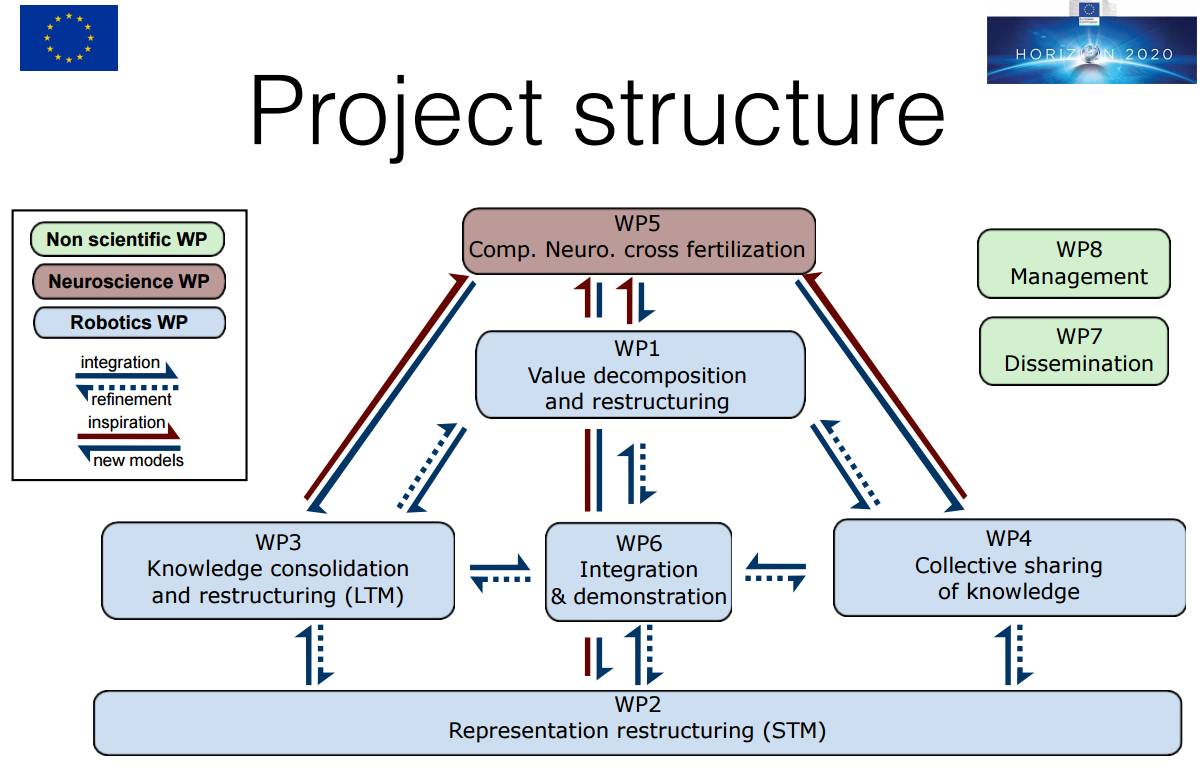
\includegraphics[width=.8\textwidth]{figures/project_structure.png}
	\label{fig:dream}
	\caption{Structure du projet Dream}
\end{figure}






\subsection{Travaux de l'équipe AMAC au sein du projet DREAM}

Une partie des membres de l'équipe AMAC travaille sur le projet DREAM (4 chercheurs, 2 post-doctorants, 3 doctorants et plusieurs stagiaires).
% Seung Su, Léni et Jonathan : tracking d'objets et création de \textit{saliency map}.

% Léni et Jonathan
Par exemple, plusieurs personnes travaillent sur la perception interactive et le tracking d'objets.
L'idée principale de ce sujet de recherche est que pour segmenter des éléments (en l'occurrence des objects manipulables) dans une scène quelconque, il n'est pas possible de se baser sur un à priori.
Pour compenser cela, le robot va interagir avec l'environnement afin d'acquérir de l'information.
% Le but d'un babillage est donc de produire une base de données.
Une première étape consiste à segmenter ce qui bouge au moment de l'interaction du robot sur les objets, tandis qu'une autre étape vise à segmenter chaque objet.
La segmentation permet d'initialiser des hypothèses d'objets (ensemble de supervoxels) avec lesquels le robot interagit afin de valider ou non l'appartenance des supervoxels à un unique objet.
% La base de données qui est construite contient pour chaque objet les exemples de supervoxels qui lui ont été attribué.
Ce babillage est orienté objet, c'est-à-dire qu'il consiste à récupérer des données à propos de chaque objet pour produire une segmentation d'objets.

% Lenni : Saliciency map babbling. Segementation à partir d'une scène.
% Peut bouger / ne peut pas bouger avec son effecteur.
%  Classificateur GMM (split and merge). Visual features (histogramme de couleur dans différents réferentiels, forme, vecteurs normaux...).

% Carlos : Apprentissage d'affordance
% Pierre : reconnaissance de formes ?

% Seungsu : QD Search, lancer de balle. Utilisation de QD Search : plus riche et divers mouvement de lancer, mouvement de haute qualité (minimisation d'énergie).
% Comportement = f(genotype)
D'autres travaux se concentrent sur le lancer de balle dans un seau, effectué par un robot.
Pour cela, des algorithmes de Quality Diversity Search sont employés.
Ces algorithmes permettent des mouvements de lancer plus riches, plus divers et de plus haute qualité en minimisant l'énergie nécessaire au lancer.

% Paul
Un autre sujet se focalise sur l'étude du chant chez le diamant mandarin.
Cet oiseau a la particularité de pouvoir apprendre le chant de son tuteur.
Il est par ailleurs communément employé en tant que modèle de l'acquisition de la parole.
Plus particulièrement, ce sujet traite de l'impact du sommeil sur l'apprentissage du chant.
% Chant unique, trajectoire d'apprentissage, qualité.
Les résultats préliminaires ont montré que l'on pouvait observer une baisse de performance durant le sommeil, à court terme donc, mais qu'il y avait en revanche une  augmentation de la performance en toute fin d'apprentissage.

% Lise
Enfin, d'autres travaux sont effectuées sur les replays (forward et backward) et se basent sur l'algorithme Dyna-Q et sur l'apprentissage par renforcement (notamment le Q-learning) pour résoudre des tâches de navigation.


\section{\'Etat de l'art}

\subsection{Affordances}

L'apprentissage des affordances est une étape cruciale dans l'approche de la robotique développementale.

% Définition
Le terme a été introduit en 1966 dans le domaine de la psychologie par J.J. Gibson comme \textit{what it offers the animal, what it provides or furnishes, either for good or for ill} \cite{opac-b1085639}.
Cette définition établit une relation forte entre un objet, une action et l'effet de cette action sur l'objet dans un environnement donné (voir Figure \ref{fig:affordances}).
En d'autres termes, une affordance est la connaissance qu'une action donnée sur un objet donné produit un certain effet.
L'idée principale derrière ce terme est d'être capable de découvrir les différentes actions qui peuvent être réalisées sur un objet, en considérant les capacités disponibles et l'environnement dans lequel s'effectue ces actions.
Les 3 composants d'une affordance sont la perception de l'objet, l'action réalisée par l'agent et l'effet résultant de cette action sur l'objet \cite{Sahin2007}.

Ce concept a influencé toutes sortes de domaines, de la robotique à l'interaction Homme-Machine en passant par le design.
Les chercheurs se sont inspirés de ce concept d'affordances pour le transposer dans le domaine de la robotique afin d'améliorer les capacités perceptives des robots \cite{Jamone2016}.
En effet, les affordances sont importantes en robotique dans la mesure où elles donnent une représentation des propriétés des objets, nécessaires pour acquérir une connaissance des actions réalisables \cite{Montesano2008}.

Dans \cite{Fitzpatrick2003}, Fitzpatrick et al. proposent une méthode permettant à un robot de découvrir et d'apprendre des affordances.
Celle-ci consiste à permettre au robot d'effectuer des actions sur un objet et d'en observer le résultat.

\begin{figure}
% \begin{wrapfigure}{r}{0.5\textwidth}
  \centering
  \begin{tikzpicture}[->,>=stealth',shorten >=1pt,auto,node distance=3.5cm,thick,main node/.style={circle,draw,minimum size=17mm,font=\Medium\bfseries}]

    \node[main node] (1) {Actions};
    \node[main node] (2) [below left of=1] {Objets};
    \node[main node] (3) [below right of=1] {Effets};

    \draw[<->] (1) edge  node[sloped, above] {} (2);
    \draw[<->] (2) edge  node[sloped, above] {} (3);
    \draw[<->] (3) edge  node[sloped, above] {} (1);
  \end{tikzpicture}

  \label{fig:affordances}
	\caption{Affordances : relation entre \textbf{Objets}, \textbf{Actions} et \textbf{Effets}.}

\end{figure}
% \end{wrapfigure}

% Capacités différentes
Les affordances permettent de découvrir les différentes actions qui peuvent être réalisées sur un objet en fonction des capacités de l'acteur.
Par exemple, une bouteille et une tasse avec une anse peuvent toutes les deux être saisies, mais cette action nécessite différentes compétences sensorimotrices pour être réalisée, en fonction des caractéristiques de l'objet.
Autre exemple, pour un robot avec des pinces, une boîte offre les affordances \textit{déplaçable} et \textit{levable}, parmi d'autres.

% Détection
Deux  approches coexistent pour détecter les affordances.
La première est une méthode analytique qui repose sur l'analyse du modèle géométrique de l'objet considéré.
La seconde est une approche basée sur le traitement des données : les caractéristiques de l'objet considéré sont comparées à celles d'objets dont on connaît les affordances.
La détection d'affordances est un préalable à l'apprentissage d'affordances \cite{Jamone2016} ? ainsi qu'à la prédiction d'effets d'une action réalisée.

% To plan the actions, the robot will first need to understand the environment, i.e. to detect and localize which objects are present in the scene.
% Furthermore, it must also be able to identify object affordances (e.g. contain or grasp) to plan the grasp and complete the task.

% En pratique
Dans la majorité des travaux mentionnés dans la littérature scientifique, les affordances d'un objet sont apprises par un robot disposant d'un bras suivant 3 étapes : exploration de l'environnement qui aboutit à la génération d'un jeu de données, apprentissage des affordances à partir du jeux de données et basé sur différentes techniques, et enfin, la validation de l'apprentissage en faisant exécuter une série de tâches au robot.

% Identification - TODO
Par ailleurs, les affordances peuvent également être utilisées pour identifier ou reproduire des actions, telles qu'expliqué dans \cite{4399517}.
Ce concept permet donc d'identifier les conséquences d'une action, afin de les enregistrer et de les réutiliser par la suite.
Le concept d'affordance, à travers la relation étroite entre objet, action et effet implique qu'il peut être utilisé pour identifier les conséquences d'une action
Les affordances fournissent des informations à propos des conséquences d'une action.
% Peut être stockée et réutilisée dans un ensemble de tâches que le rotobot doit apprendre et réaliser.

% Planification
Les affordances peuvent être utilisées pour prédire les effets d'une action ou pour planifier les actions à effectuer.
Elles permettent également la reconnaissance d'actions et l'imitation d'actions.
En planification, les affordances sont capitales pour réaliser des actions.
Grâce à elles, le robot peut utiliser sa connaissance des affordances pour choisir la prochaine action à effectuer sur un objet afin d'accomplir une tâche.

% Actions préalables
Toutefois, il est nécessaire de spécifier au préalable un certain nombre d'actions prédéfinies élémentaires afin d'être capable de découvrir des affordances \cite{Montesano2008}.
Par exemple, cela peut concerner des actions du type \textit{Pousser} ou \textit{Soulever}.

% AfNet
Il existe une base de données open source d'affordances, AfNet\footnote{http://theaffordances.net}, contenant les définitions de caractéristiques d'affordances pour près de 250 objets communément utilisés. 




\subsection{Boostrapping}

Meltzoff et al. expliquent dans \cite{EDP:EDP157} que les enfants ne savent pas à priori quels mouvements musculaires permettent d'atteindre un état particulier.
Les auteurs appellent cela le babillage corporel, directement inspiré du babillage vocal lorsque les enfants expérimentent des sons vocaux.
Ils expliquent que les enfants font des mouvements répétés, comme dans un jeu.
Finalement, après un certain temps et de répétitions, les enfants apprennent la relation entre les mouvements qu'ils effectuent et leurs effets.
Ce concept a été réutilisé par la suite dans le domaine de la robotique développementale.
En effet, pour un robot, apprendre des affordances nécessite d'interagir avec l'environnement à travers une phase d'exploration, ce qui correspond au babillage. Différentes heuristiques existent pour effectuer cette exploration.



\subsubsection{Babillage sensorimoteur}

Le babillage sensorimoteur constitue une première heuristique.
Il existe de multiples façons de réaliser ce babillage.
Une première approche, qualifiée de naïve, consiste à utiliser des mouvements aléatoires.
Cette approche est la plus simple à implémenter mais elle présente un défaut majeur : elle peut générer un nombre important de mouvements qui ne produisent pas de contact avec les objets.

Une seconde approche est présentée par Maestre et al. dans \cite{Maestre2015} où ils décrivent l'utilisation de l'algorithme évolutionnaire Novelty Search.
Cet algorithme permet de générer des trajectoires permettant de maximiser l'exploration de l'environnement.
Les résultats de cet article montrent que les trajectoires permettant de toucher les objets sont de plus en plus privilégiées au fur et à mesure des générations.




\subsubsection{Motivations}

Une seconde heuristique réside dans les motivations intrinsèques.
Ce concept a été décrit par Ryan et Deci dans \cite{Ryan2000}, puis par Hull et plus tard formalisé en modèles computationnels par Oudeyer et Kaplan dans \cite{10.3389/neuro.12.006.2007}.
Les motivations intrinsèques permettent d'explorer progressivement l'environnement en favorisant une spécialisation progressive des différents composants.
Dans cette optique, le concept de curiosité est davantage favorisée au profit de la recherche de la performance.
Cette heuristique est utilisé en robotique et spécifiquement en robotique développementale.


\subsubsubsection{Motivations internes et externes}

Dans le cadre d'une motivation, la récompense correspond à la valeur numérique que le système doit maximiser.
Lorsque la récompense provient de l'extérieur du système, il est question de motivation externe.
En revanche, si la valeur à maximiser est calculée de façon interne, alors il s'agit de motivation interne.

\subsubsubsection{Motivations intrinsèques et extrinsèques}

Ryan et Deci définissent les motivations intrinsèques comme des activités amusantes ou comprenant du défi.
D'autre part, ils définissent les motivations extrinsèques par des activités réalisées pour atteindre un résultat.

Pour Oudeyer et al., les notions de \og{}amusant\fg{}, \og{}défi\fg{} ou de \og{}nouveauté\fg{} n'ont pas de définitions claires et explicites dans le domaine de l'informatique.
Ces définitions sont vagues et peuvent être interprétées de différentes façons.
Par ailleurs, le concept de résultat est ambigu.

Pour Oudeyer et al. , les motivations intrinsèques et extrinsèques ne sont pas exclusives : une même tâche peut concilier ces deux types de motivations.
Ils définissent par ailleurs deux modèles de motivations intrinsèques.
Le premier est basé sur les connaissances.
Il vise à mesurer les dissonances entre la situation expérimentée par le robot et les connaissance et attente que le robot a de ces situations.
Le deuxième est basé sur les compétences. Il mesure les compétences qu'un agent a pour réaliser des résultats ou objectifs fixé par lui-même.




\subsection{Réseaux bayésiens}

Une fois que le babillage sensorimoteur a été réalisé, les relations entre objets, actions et effets nécessitent d'être modélisées.
Les réseaux bayésiens constituent une méthode efficace pour réaliser cela. 
Les réseaux bayésiens sont des modèles graphiques probabilistes représentés sous la forme de graphe dirigés et acycliques.
Les noeuds représentent les variables aléatoires et les liens représentent l'influence entre les variables.
Leur intérêt réside dans la possibilité offerte de combiner les connaissances des experts, contenues dans le graphe, et l'expérience, contenue dans les données.

Dans \cite{Montesano2008}, Montesano et al. présentent un modèle de réseau bayésien dans lequel les dépendances entre objets, actions et effets sont modélisées.
Une des motivations des auteurs réside dans le fait de pouvoir permettre à un robot d'apprendre des actions par imitation.
Ce modèle de réseau bayésien permet donc d'apprendre des affordances concernant des objets mais il permet également de prédire des actions en fonction des effets obtenus.
En effet, ce type de modèle est capable de réaliser des inférences et sa représentation des affordances comme dépendances probabilistes permet d'analyser et de comprendre les résultats d'apprentissage.

La planification de tâches est une autre utilisation possible des réseaux bayésiens modélisant des affordances.
Gonçalves et al. présentent un autre framework utilisant les réseaux bayésiens \cite{Goncalves2014} pour planifier une tâche en fonction des effets attendus.
Le robot considéré dans l'article dispose de différents objets utilisables en tant qu'outils et différentes actions dans son répertoire.
Il peut raisonner à partir de ceux-ci pour atteindre les effets désirés sur un objet grâce à des objets devant lui dont certains lui sont peut-être inconnus.
Par exemple, à partir d'un ensemble d'objets disponibles de type \textit{outil} ainsi que d'un effet désiré (amener plus près) sur un objet, un robot disposant d'un réseau bayésien de ce type peut raisonner pour trouver quel outil et quelle action disponibles sont les plus efficaces pour réaliser l'effet désiré.




\subsection{Réseaux de neurones}

Les réseaux de neurones constituent une autre approche pour détecter les affordances.
Nguyen et al. proposent dans \cite{Nguyen2017} un nouveau framework basé sur l'utilisation de réseaux de neurones convolutionnels profonds pour détecter des affordances.
Une forme 3D englobant les objets est générée et permet à ce réseau de neurones d'apprendre ses caractéristiques de profondeur de ces formes englobantes.
L'expérimentation décrite dans cet article est réalisée sur des images d'images du monde réel contenant des objets usuels.
Cette méthode est initialement grossière mais devient de plus en plus fine au cours du temps.



\subsection{Utilisation d'outils}

Au-delà des affordances, des recherches prometteuses se concentrent sur la manipulation d'outils.
Dans \cite{Montesano2008}, Montesano et al. proposent une approche pour apprendre les affordances visuelles d'objets ou d'outils.
Dans cet article, un robot apprend les caractéristiques visuelles d'objets et d'outils à l'aide de descripteurs visuels.
De cette façon, ils montrent que le robot est capable de réaliser une action spécifique ou d'obtenir un résultat désiré.
L'utilisation des descripteurs visuels permet au robot de généraliser avec des objets inconnus.

D'autre part, Gonçalves et al. \cite{Goncalves2014} propose un modèle probabiliste capable d'apprendre les interactions mutuelles entre objets dans des tâches complexes qui impliquent une manipulation.
Dans ces tâches, l'un des objets devient un outil une fois saisi et utilisé, tandis que l'autre objet est celui sur lequel l'outil agit.
Avec ce modèle, le robot considéré est capable d'apprendre des relations porteuses de sens entre actions, outils, d'autres objets et les effets associés, ainsi que d'exploiter la connaissance acquise pour faire des prédictions et prendre des décisions optimales.




\subsection{Algorithmes de clusterisation}

Le clustering ou partitionnement de données fait partie du domaine de l'analyse de données.
Cette technique a été développée pour traiter des jeux de données trop massifs et trop complexes pour être traités manuellement.
L'idée est de grouper un ensemble d'objets de telle manière à ce que les objets présents au sein d'un même cluster soit le plus similaire possible tandis que les différences entre les différents clusters soient les plus grandes possibles afin d'obtenir une séparation nette entre clusters.
Le clustering est considéré comme une des questions les plus importantes en apprentissage non supervisé, c'est-à-dire sans connaissance préalable sur la classification des objets \cite{Xu2015}, \cite{Andreopoulos2009}, \cite{Fahad2014}, \cite{Tan2005} et \cite{Sajana2016}.

Les variables utilisées dans le clustering peuvent être discrètes, binaires, nominales ou ordinales.

Différentes notions de mesure de distance (ou dissimilarité) existent. Parmi celles-ci, il est possible de citer :

\begin{enumerate}
  \item Distance de Minkowski
  \item Distance euclidienne
  \item Distance cosine
  \item Distance de Mahalanobis
  \item Distance moyenne
\end{enumerate}

La qualité d'un clustering dépend donc de la mesure de distance utilisée.

Différentes typologies de clustering existent. Voici quelques exemples : 

\begin{enumerate}
  \item Partition : initialement, les éléments sont considérés comme faisant partie d'un seul cluster. Puis les éléments initiaux sont groupés de façon itérative en différentes partitions dont le nombre est donné en paramètre en entrée ;
  \item Connectivité (hiérarchique) : ce type de clustering partitionne les éléments dans un arbre où chaque noeud de l'arbre représente un cluster ;
  \item Distribution : les clusters sont modélisés en utilisant une distribution statistique ;
  \item Densité : un cluster est une région dense d'objets entourée d'une région de faible densité. Les éléments présents dans les zones de faible densité sont considérés comme du bruit ;
  \item Grille : les données sont partitionnées en un nombre de cellules formant une structure de grille.
  % \item : graphe
\end{enumerate}



\subsection{Algorithmes génétiques}
 
L'évolution biologique peut être considérée comme un mécanisme d'optimisation qui vise à permettre aux meilleurs individus de survivre dans leur environnement.
Afin de résoudre des problèmes d'optimisation difficiles, le concept d'algorithme génétique a été proposé par John Holland et son équipe \cite{Holland:1975} dans les années 1970. 
Les algorithmes génétiques s'inspirent donc de l'évolution biologique et se basent sur des mécanismes similaires d'évolution.
Ils ne visent pas à trouver une solution exacte au problème posé mais plutôt à trouver une solution qui satisfait le plus aux différents critères.
Par ailleurs, ils s'appliquent surtout à des problèmes qui ne sont pas résolvables en temps raisonnable avec des méthodes analytiques ou algorithmiques classiques.
Le calcul s'effectue en parallèle sur une population d’individus initialisée aléatoirement qui correspondent aux solutions potentielles au problème posé. 
La génération de nouveaux individus s'effectue grâce à différents d’opérateurs d’exploration de l'espace de recherche. 
Le croisement consiste en la création d’un nouvel individu à partir de plusieurs autres individus. 
La mutation vise à la modification aléatoire d’une partie de l’individu. 
Enfin, chaque individu est évalué à l'aide d'une fonction coût et les individus les plus performants sont sélectionnés parmi la population courante d'individus.
Ces cycles d'évolutions sont répétés tant qu'une solution correcte n'a pas été trouvée.
Un individu contient un génotype qui est encodé sous la forme de flottants, de chaîne de caractères ou d'entiers.

Les algorithmes génétiques multi-objectifs sont une variante des algorithmes génétiques classiques.
Ils sont utilisés lorsque le problème posé comporte plusieurs objectifs à optimiser.
Les solutions à ce problème ne sont pas uniques mais sont définies en un ensemble de solutions optimales, localisées sur le front de Pareto de l'espace des solutions.
Elles constituent donc un ensemble de solutions optimales au regard des différents paramètres optimisés.
L'algorithme NSGA-II\cite{Deb:2002:FEM:2221359.2221582} est une version améliorée de NSGA et repose sur 3 principes.
Tout d'abord, il favorise l'élitisme : seuls les meilleurs individus parmi les parents et les enfants sont gardés.
Il favorise par ailleurs les solutions non dominées et enfin, il utilise une variété explicite de solutions.

Ces algorithmes génétiques ont des domaines d'applications très variés : optimisation, apprentissage ou étude du vivant.


% \subsection{Related work}

% Ce stage de fin d'études l'a été dans le cadre du projet DREAM, débuté en 2015. Ce projet implique 5 partenaires académiques: UMPC/CNRS (coordinateur), ENSTA ParisTech, Universidade da Coruña, Vrije Universiteit Amsterdam et Queen Mary University of London. Ces différents acteurs ont différents rôles au sein du projet DREAM. See waves.

% \`A l'issue du projet DREAM, les différents modules doivent permettre de constituer un ensemble.
% % At the end of the DREAM project, the different modules are aimed at be linked together.

% Our work is directly based on actual PhD student's work on learning affordances inspired from motor babbling.

% Linkedin: "The main goal of this thesis is the autonomous creation by a robot of a minimal directory of concepts related to its morphology, its environment, and the accomplished tasks executed. The robot must be able to build and update its internal world model through interactions with its environment (cognitive bootstrapping). This work follows the approach proposed in developmental robotics, inspired by the development of the infants, where abstract concepts are created progressively based on the sensori-motor capabilities of an agent.

% Executed in an iterative loop, a dataset is created by the robot through the babbling of its environment; some candidate world models are defined based on the data gathered; and a new dataset is created, in order to discriminate these models, improve them and generate new simpler ones."




\section{Notre travail}


\subsection{Environnement}

\begin{figure}
  \begin{center}
    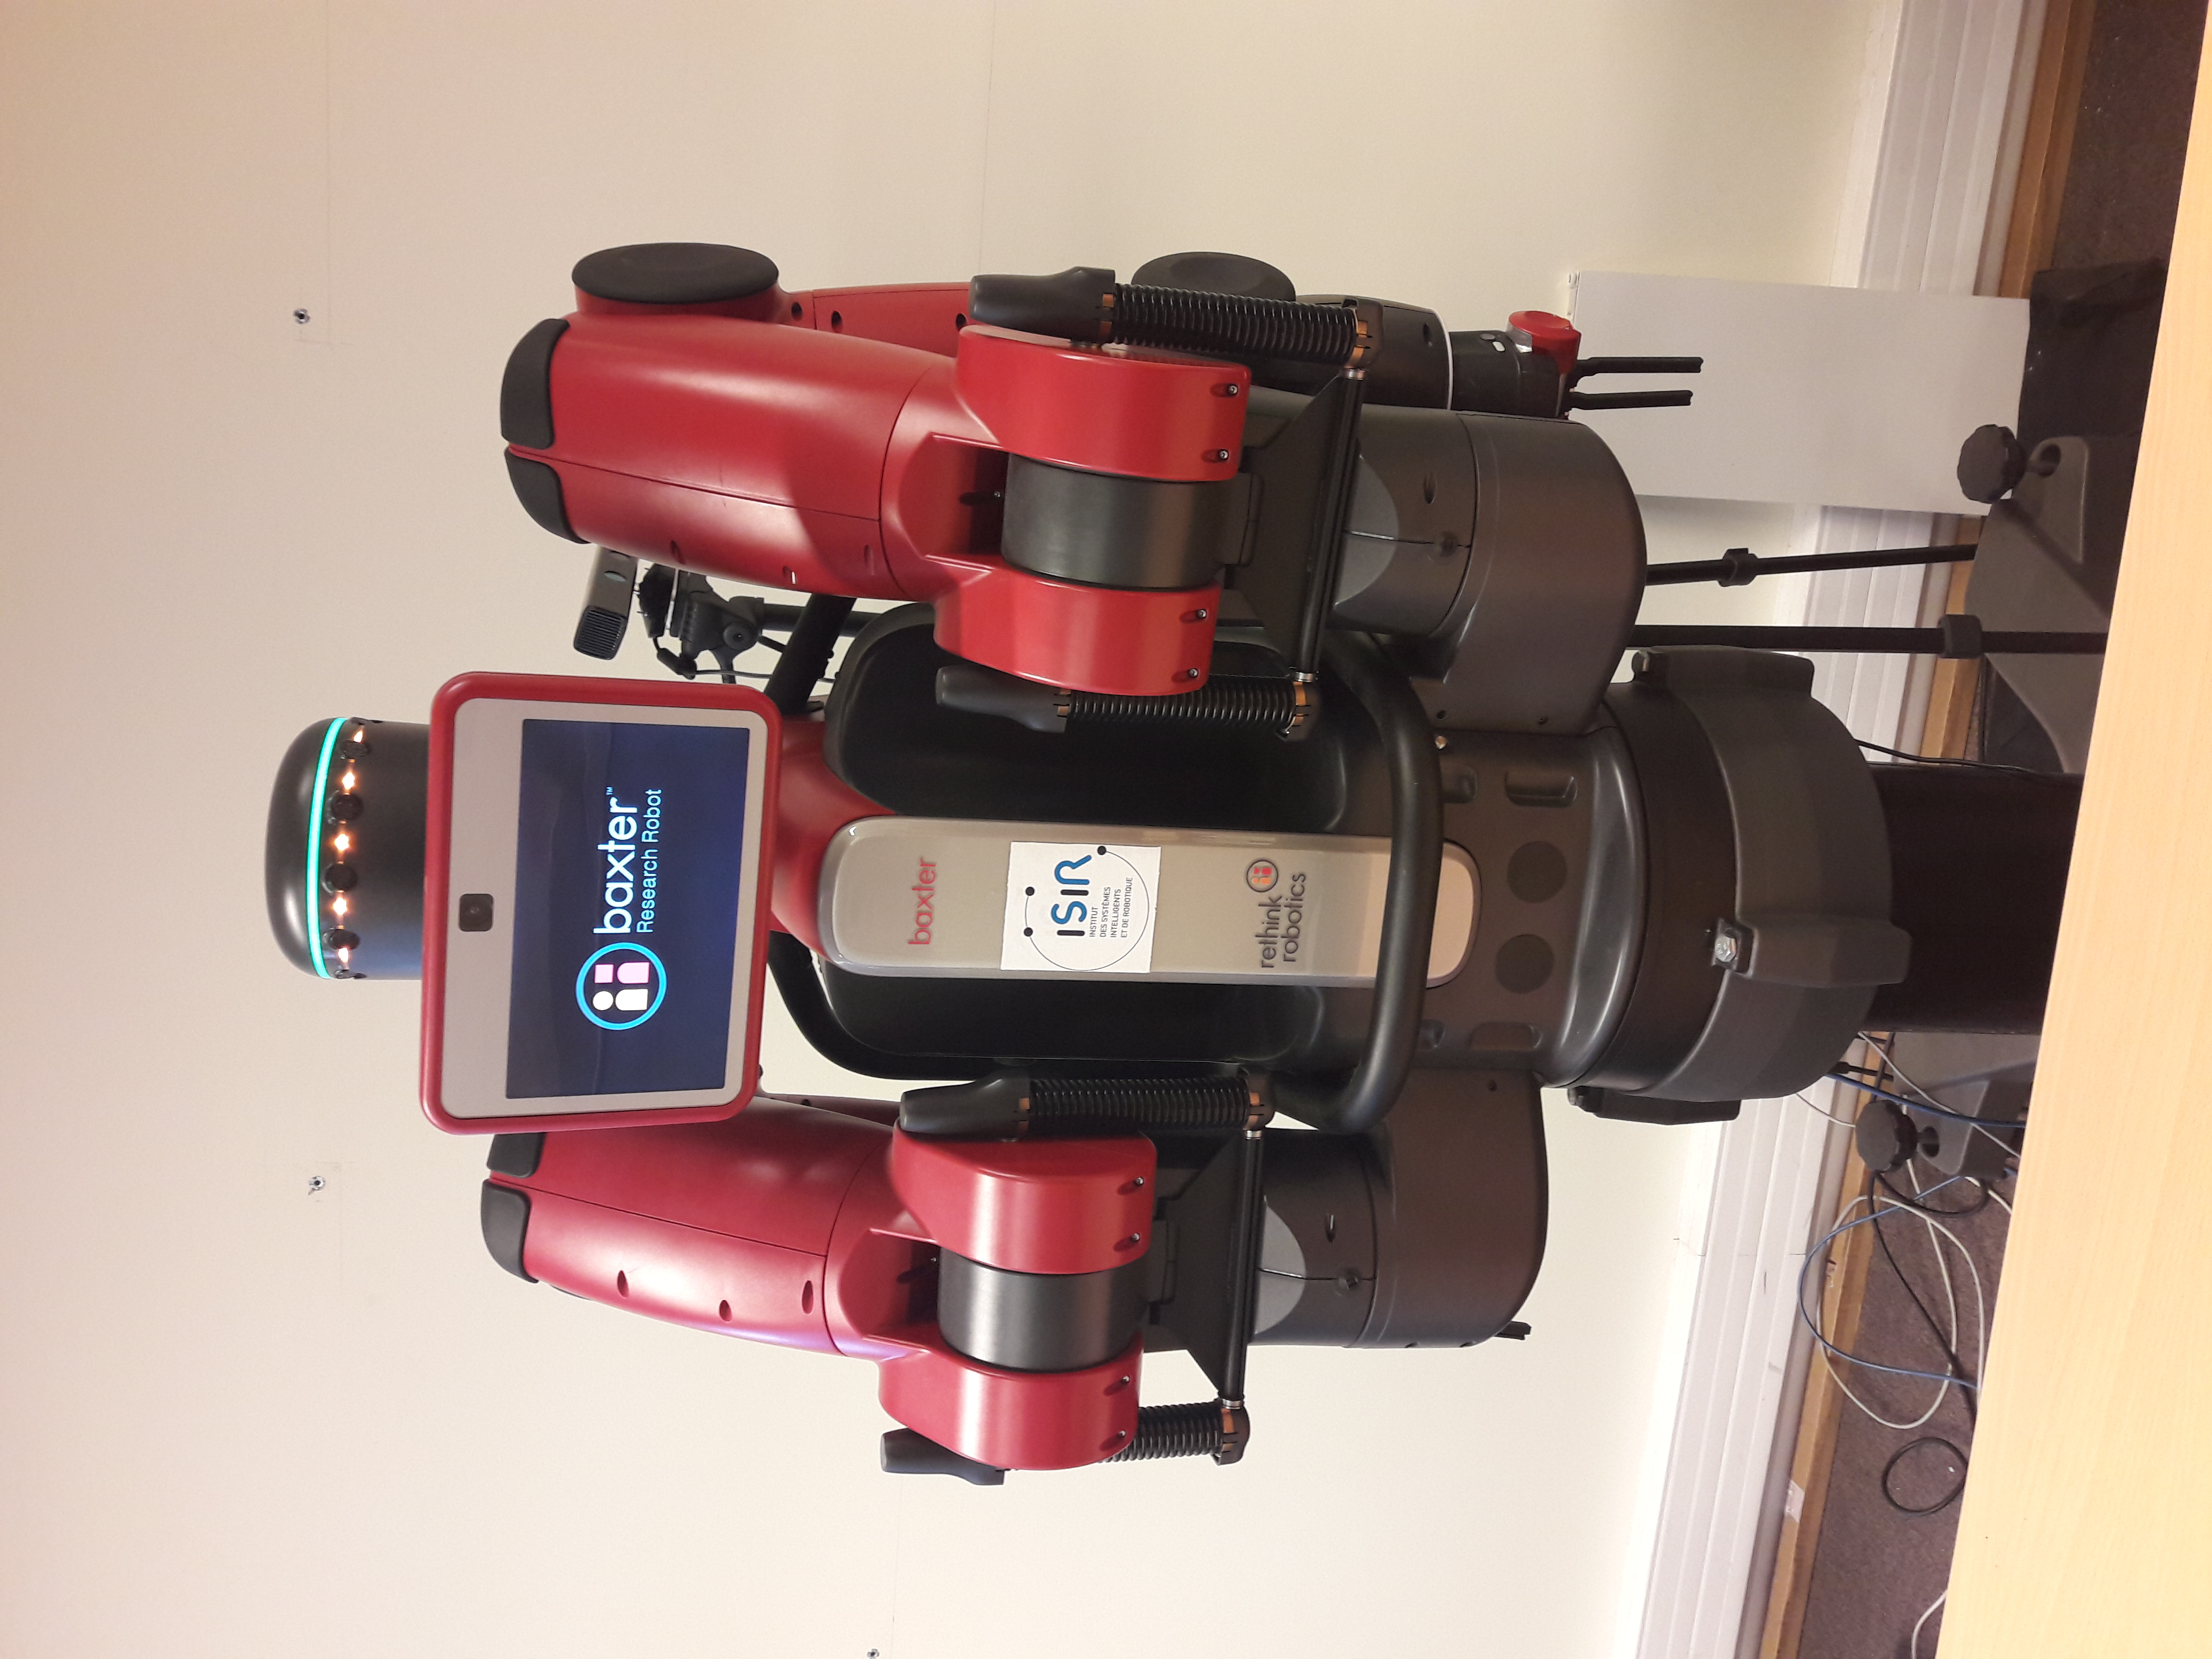
\includegraphics[angle=-90, width=0.4\textwidth]{figures/baxter}
  \end{center}
  \caption{Le robot Baxter de Rethink Robotics utilisé à l'ISIR.}
  \label{fig:baxter}
\end{figure}

\lettrine{A}{fin} de développer des algorithmes d'intelligence artificielle dans le domaine de la robotique, il est nécessaire de disposer d'une multitude d'outils tels qu'un simulateur et un framework pour communiquer avec les différents composants, en plus de disposer, tout naturellement, d'un robot.

% \begin{wrapfigure}{r}{0.45\textwidth}
%   \begin{center}
%     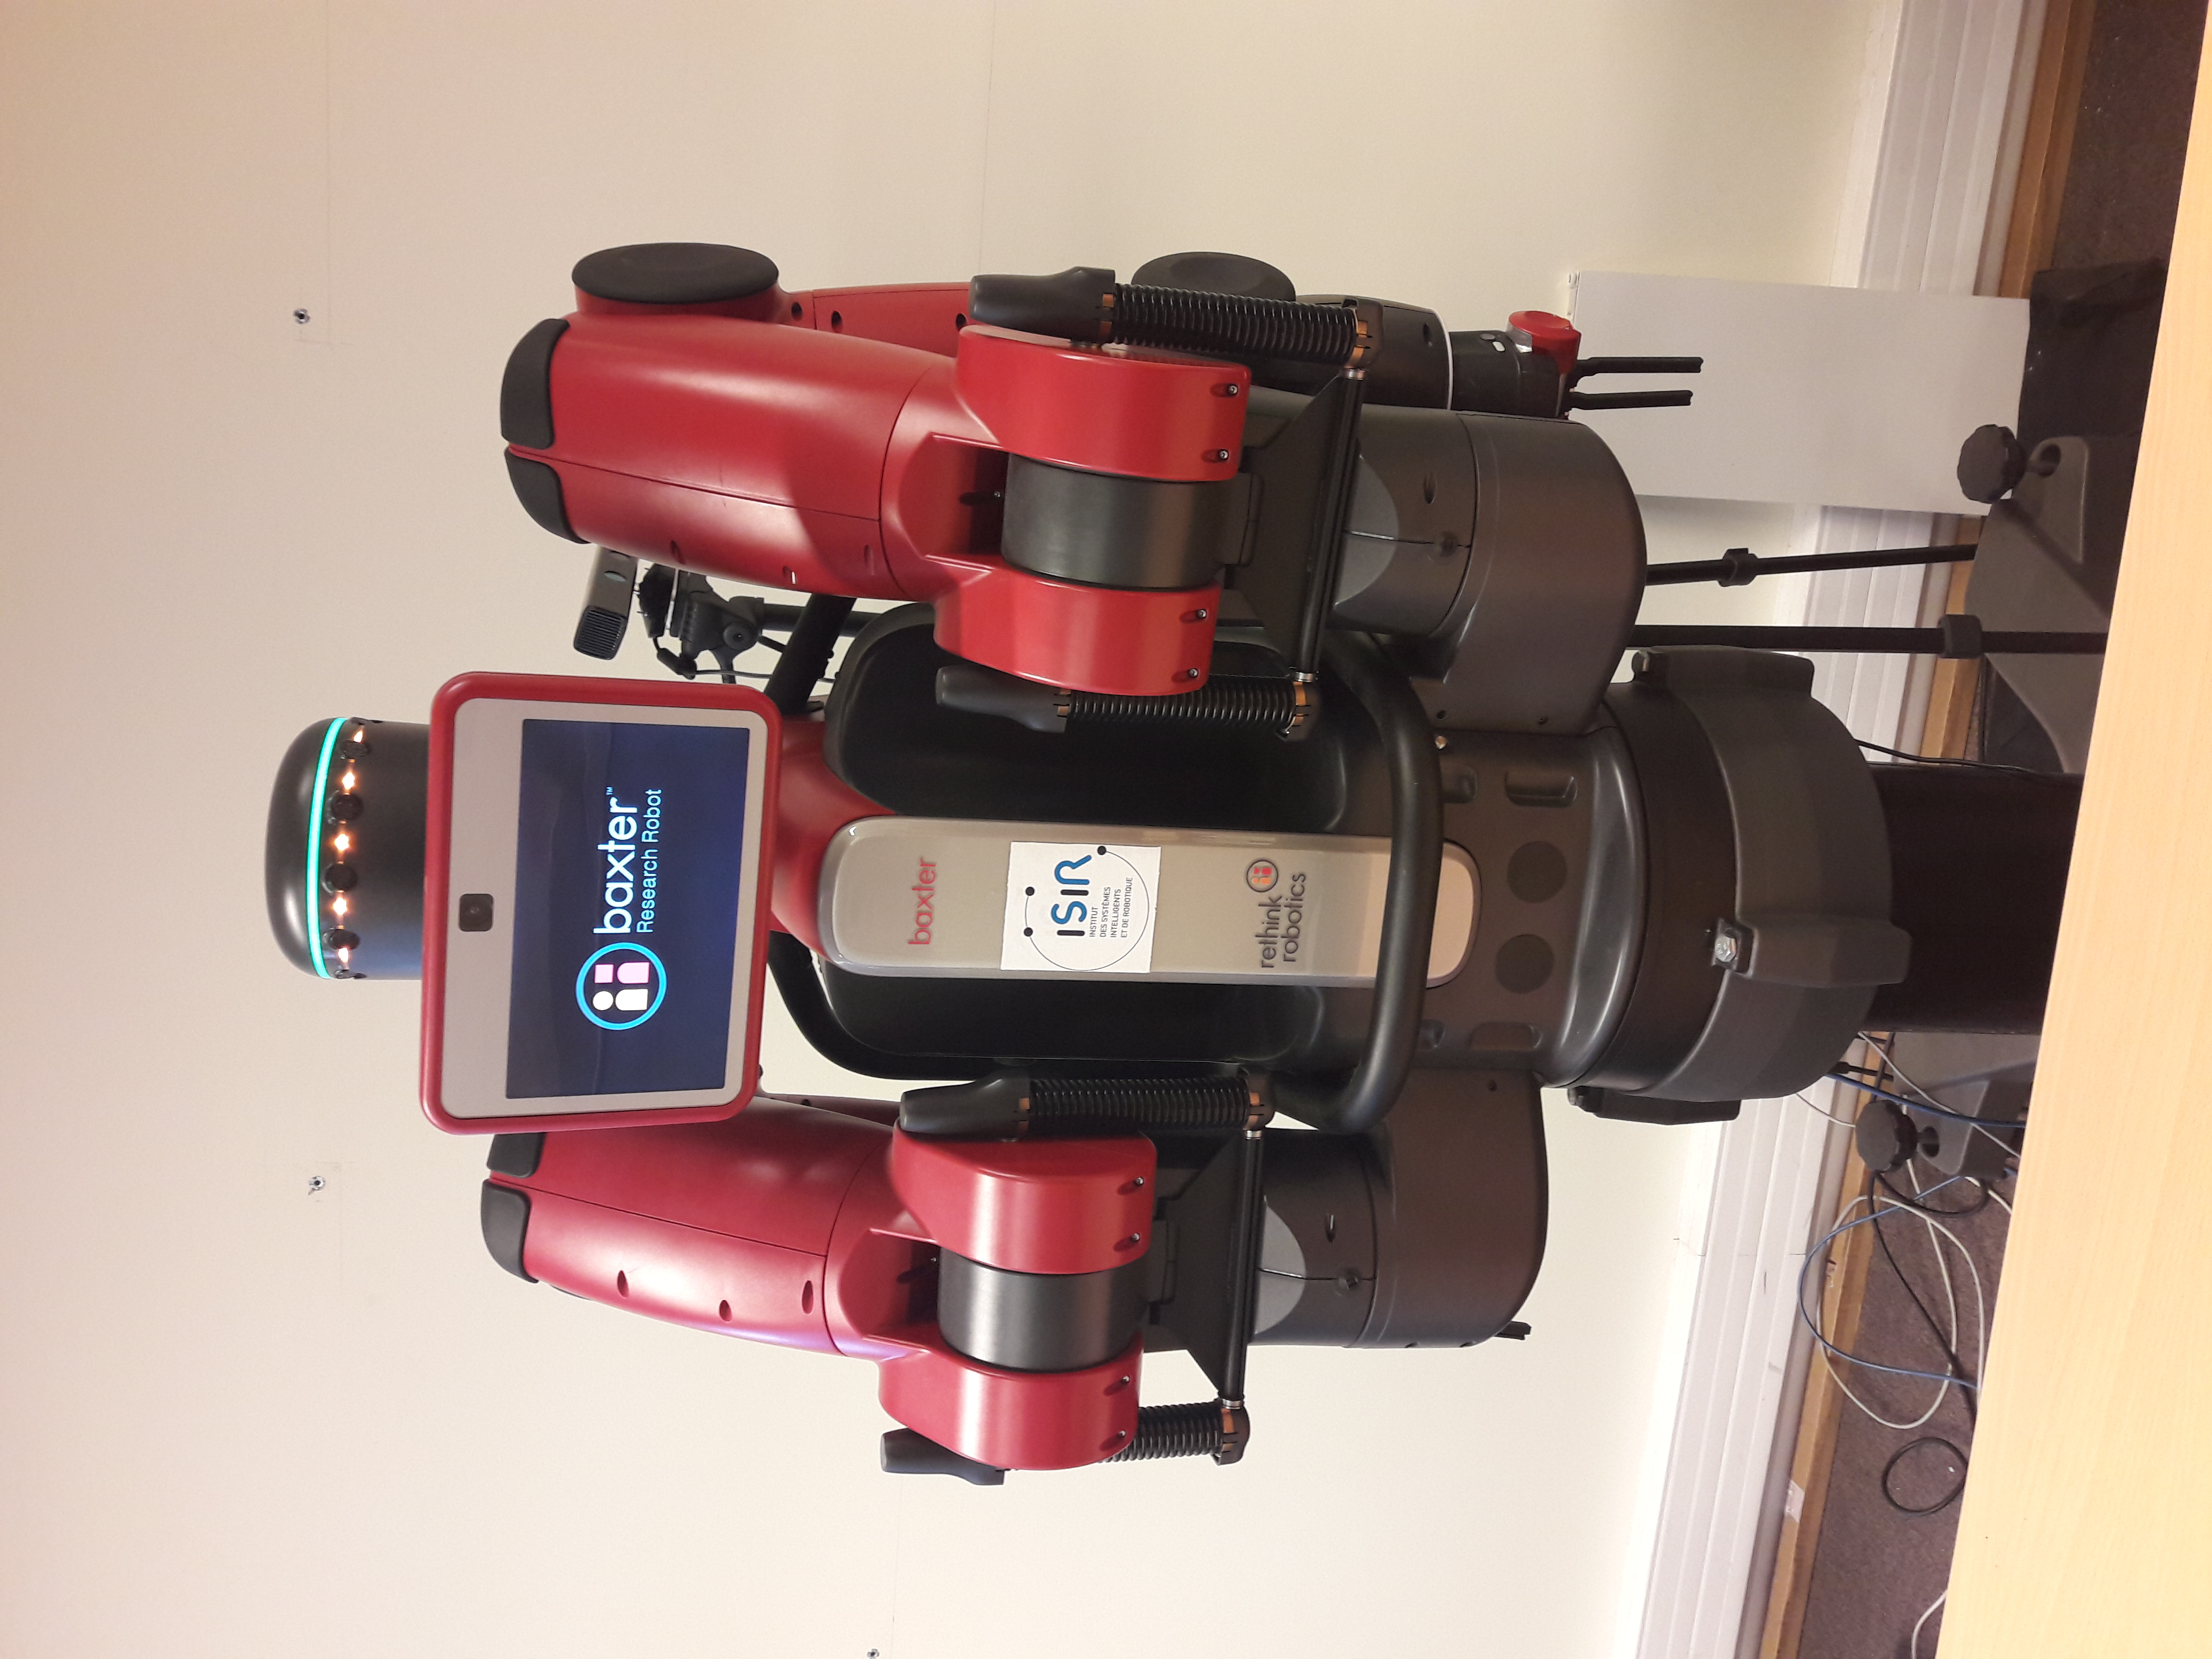
\includegraphics[angle=-90, width=0.4\textwidth]{figures/baxter}
%   \end{center}
%   \caption{Le robot Baxter de Rethink Robotics utilisé à l'ISIR.}
%   \label{fig:baxter}
% \end{wrapfigure}

Dans le cadre du projet DREAM, l'ISIR bénéficie du robot Baxter\footnote{http://www.rethinkrobotics.com/baxter/tech-specs/} (voir figure \ref{fig:baxter}).
C'est un robot développé par Rethink Robotic et utilisé à la fois à des fin industrielles et de recherche.
Ce robot antropormorphique à deux bras dispose d'un \og{}visage animé\fg{} et de deux fois sept degrés de liberté et de multiples senseurs\footnote{http://sdk.rethinkrobotics.com/wiki/Hardware\_Specifications}.
En plus d'être programmable par le biais d'un code source, il est possible de lui faire apprendre la réalisation de tâches en guidant ses bras et effecteurs lors d'une phase de programmation gestuelle.

Gazebo\footnote{http://gazebosim.org} est un simulateur nécessaire pour valider le bon comportement du robot et éviter ainsi tout problème en situation réelle.
La figure \ref{fig:setup} donne un aperçu d'une simulation lancée avec Gazebo.

MoveIt!\footnote{http://moveit.ros.org} est un framework open source conçu pour la manipulation de robots et inclut de nombreux composant de planification de mouvements, manipulation, perception 3D, cinématique, contrôle et navigation.
Ce framework permet de de développer facilement des applications robotiques complexes.

ROS\footnote{http://www.ros.org/} est un framework flexible pour contrôler un robot.
Il comporte différents outils, bibliothèques de fonctions et permet l'interaction et la communication de tous les composants, notamment sous la forme de \textit{service} (client/serveur) ou de \textit{topics} qui exposent des données (suscriber/publisher).


% \begin{figure}
% 	\centering
% 	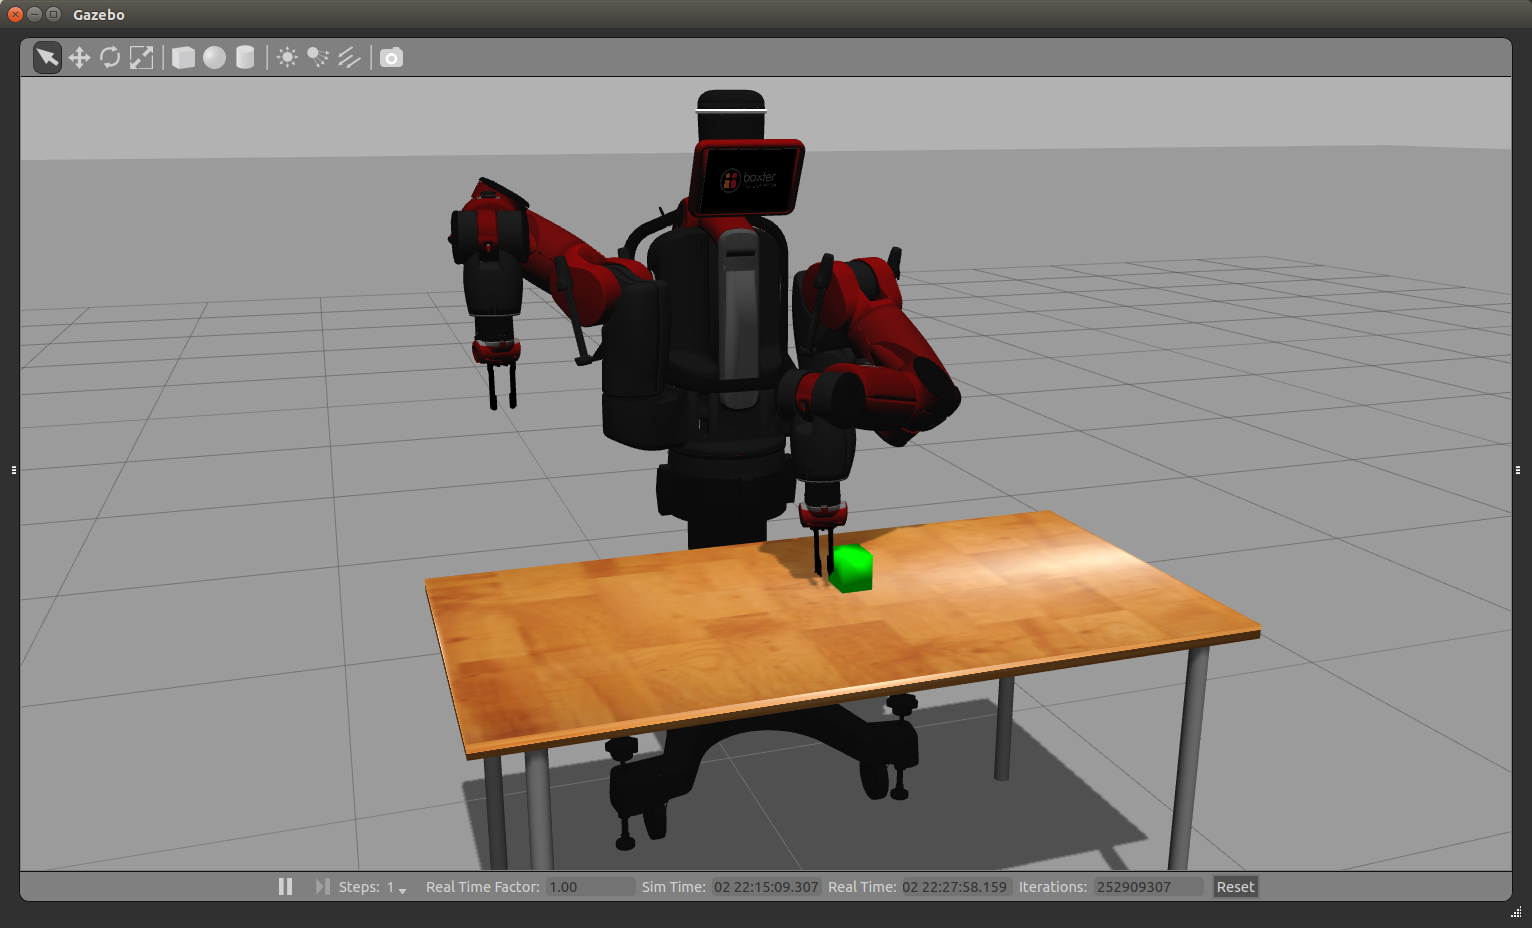
\includegraphics[width=\textwidth]{figures/gazebo}
% 	\label{fig:gazebo}
% 	\caption{Gazebo simulator}
% \end{figure}




\subsection{Discrétisation adaptative}


\subsubsection{Travaux relatifs}

Notre travail se base en partie sur les travaux existants d'un doctorant, intégré également dans le projet DREAM, et portant sur la découverte des affordances.
Dans ces travaux, le nombre d'actions disponibles et connues par le robot est arbitrairement paramétré (par exemple : \textbf{Gauche}, \textbf{Droite}, \textbf{Haut}, \textbf{Bas}). La figure~\ref{fig:trajectories} montre ces quatre effets réalisables par le robot en simulation.

% \begin{wrapfigure}{r}{0.5\textwidth}
%   \begin{center}
%     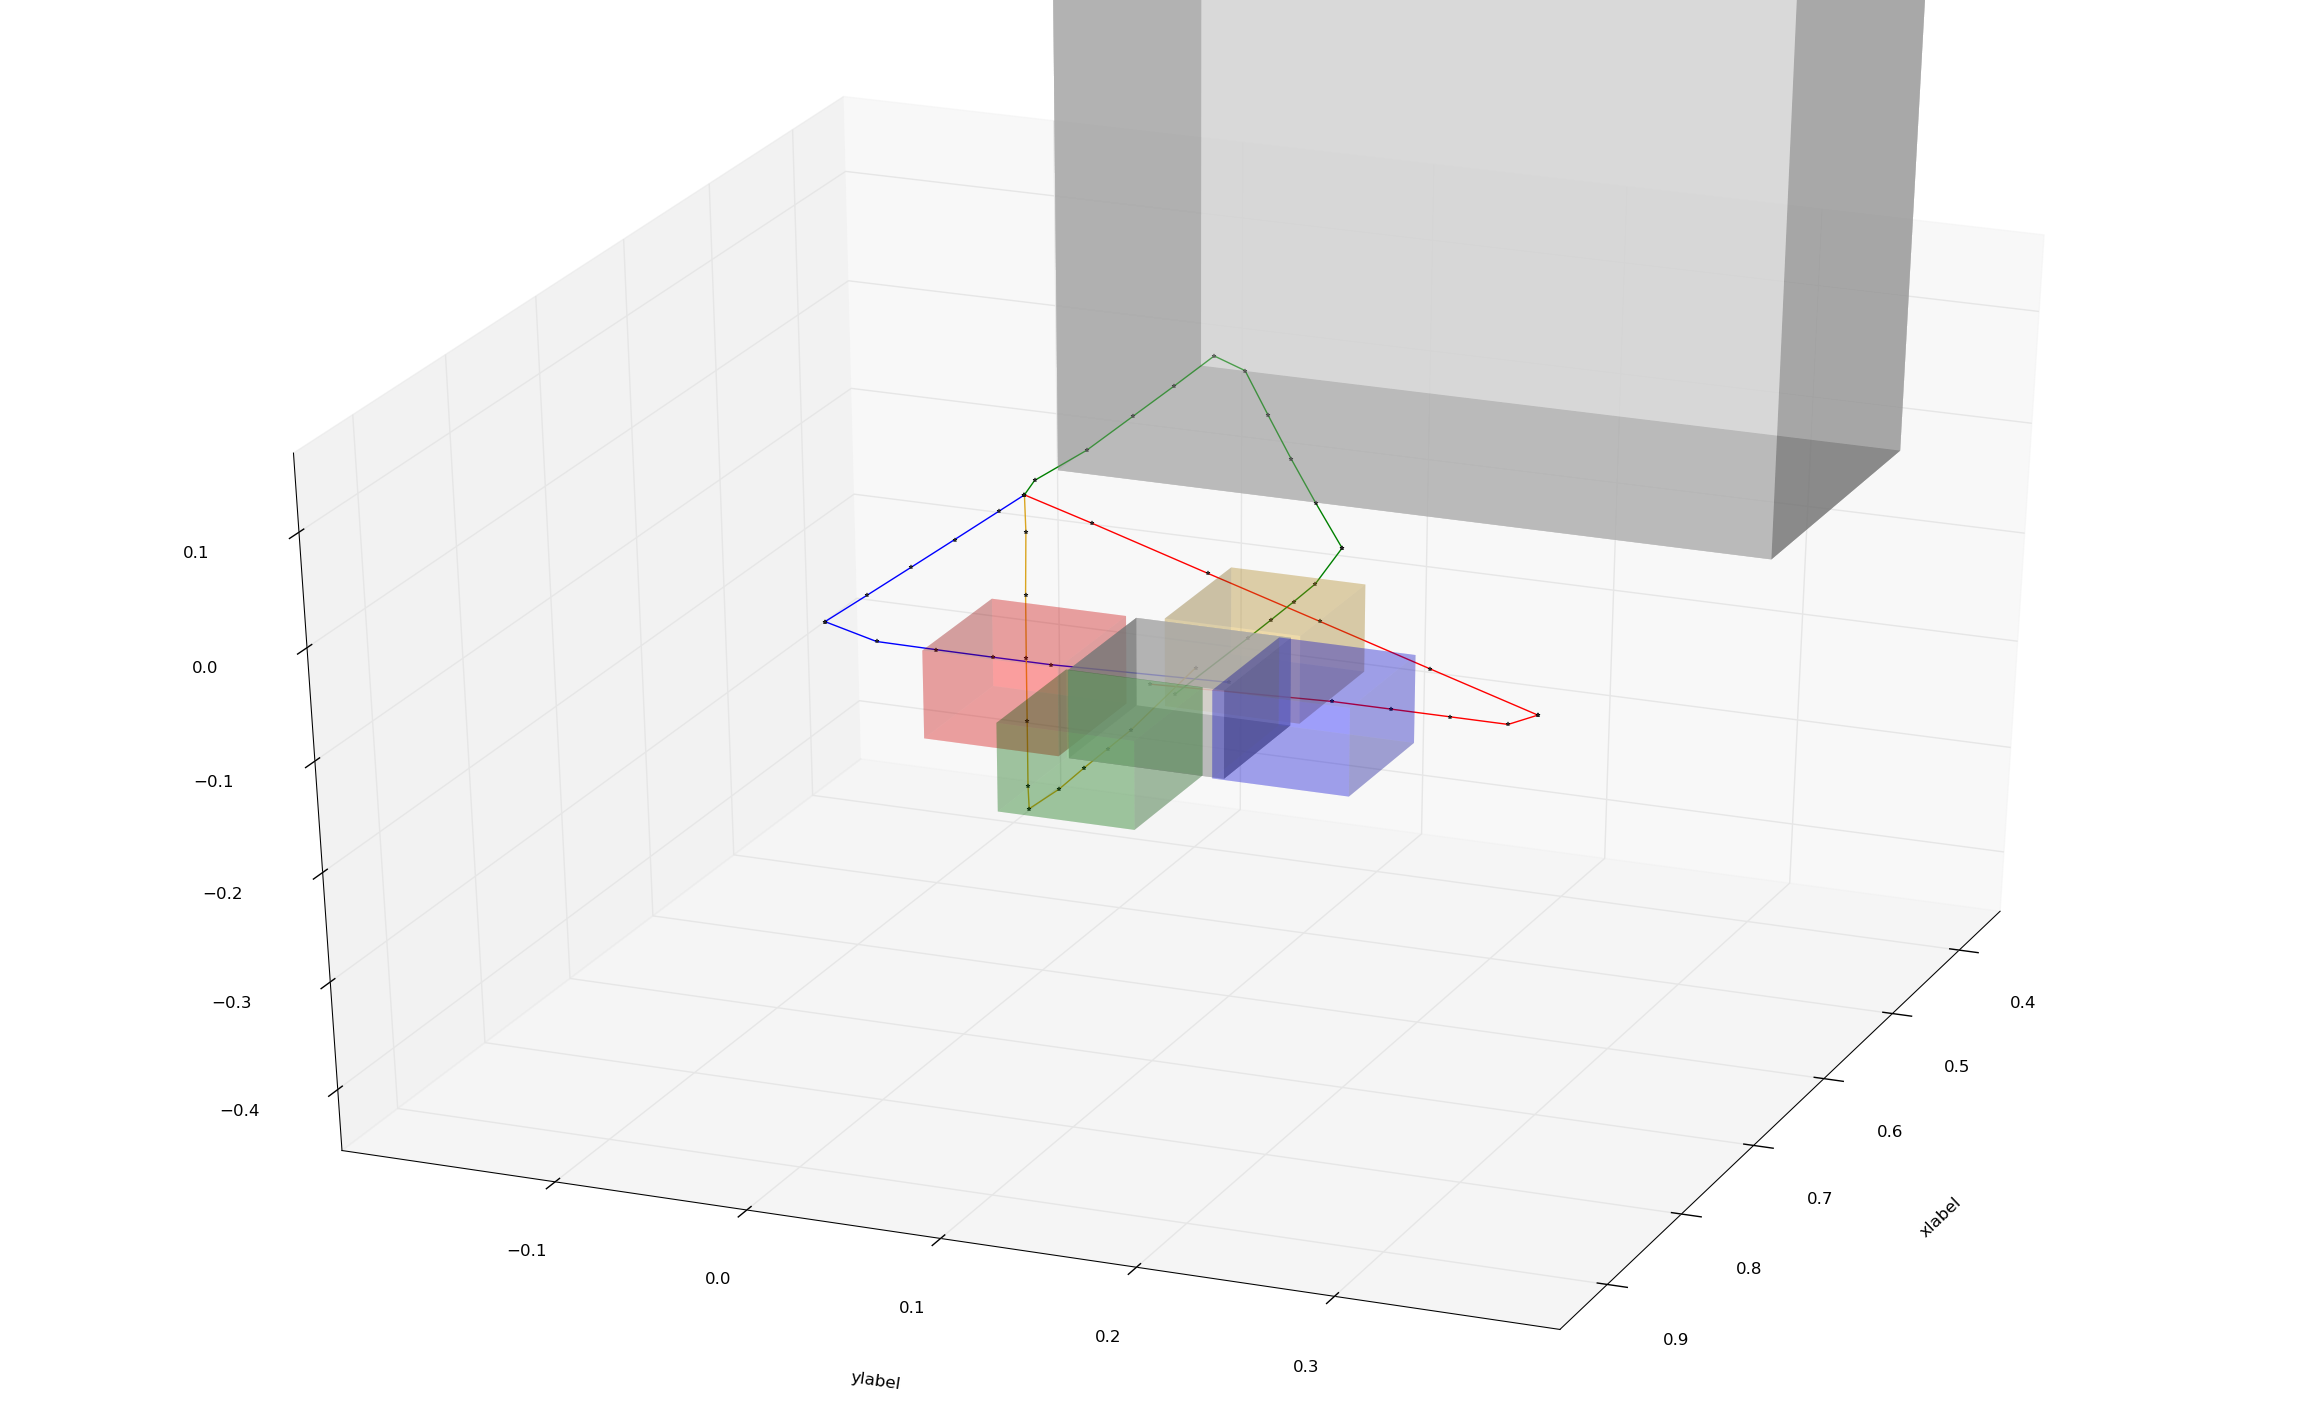
\includegraphics[width=0.48\textwidth]{figures/trajectories}
%   \end{center}
%   \caption{Différentes trajectoires réalisées par le robot (représenté par le volume gris). La position initiale de l'objet est représentée par le cube gris au milieu. Chaque cube coloré correspond au mouvement de la même couleur (par exemple, le cube rouge est la position finale du cube gris après avoir poussé par l'effecteur du robot suivant la trajectoire rouge).}
%   \label{fig:trajectories}
% \end{wrapfigure}

\begin{figure}
  \begin{center}
    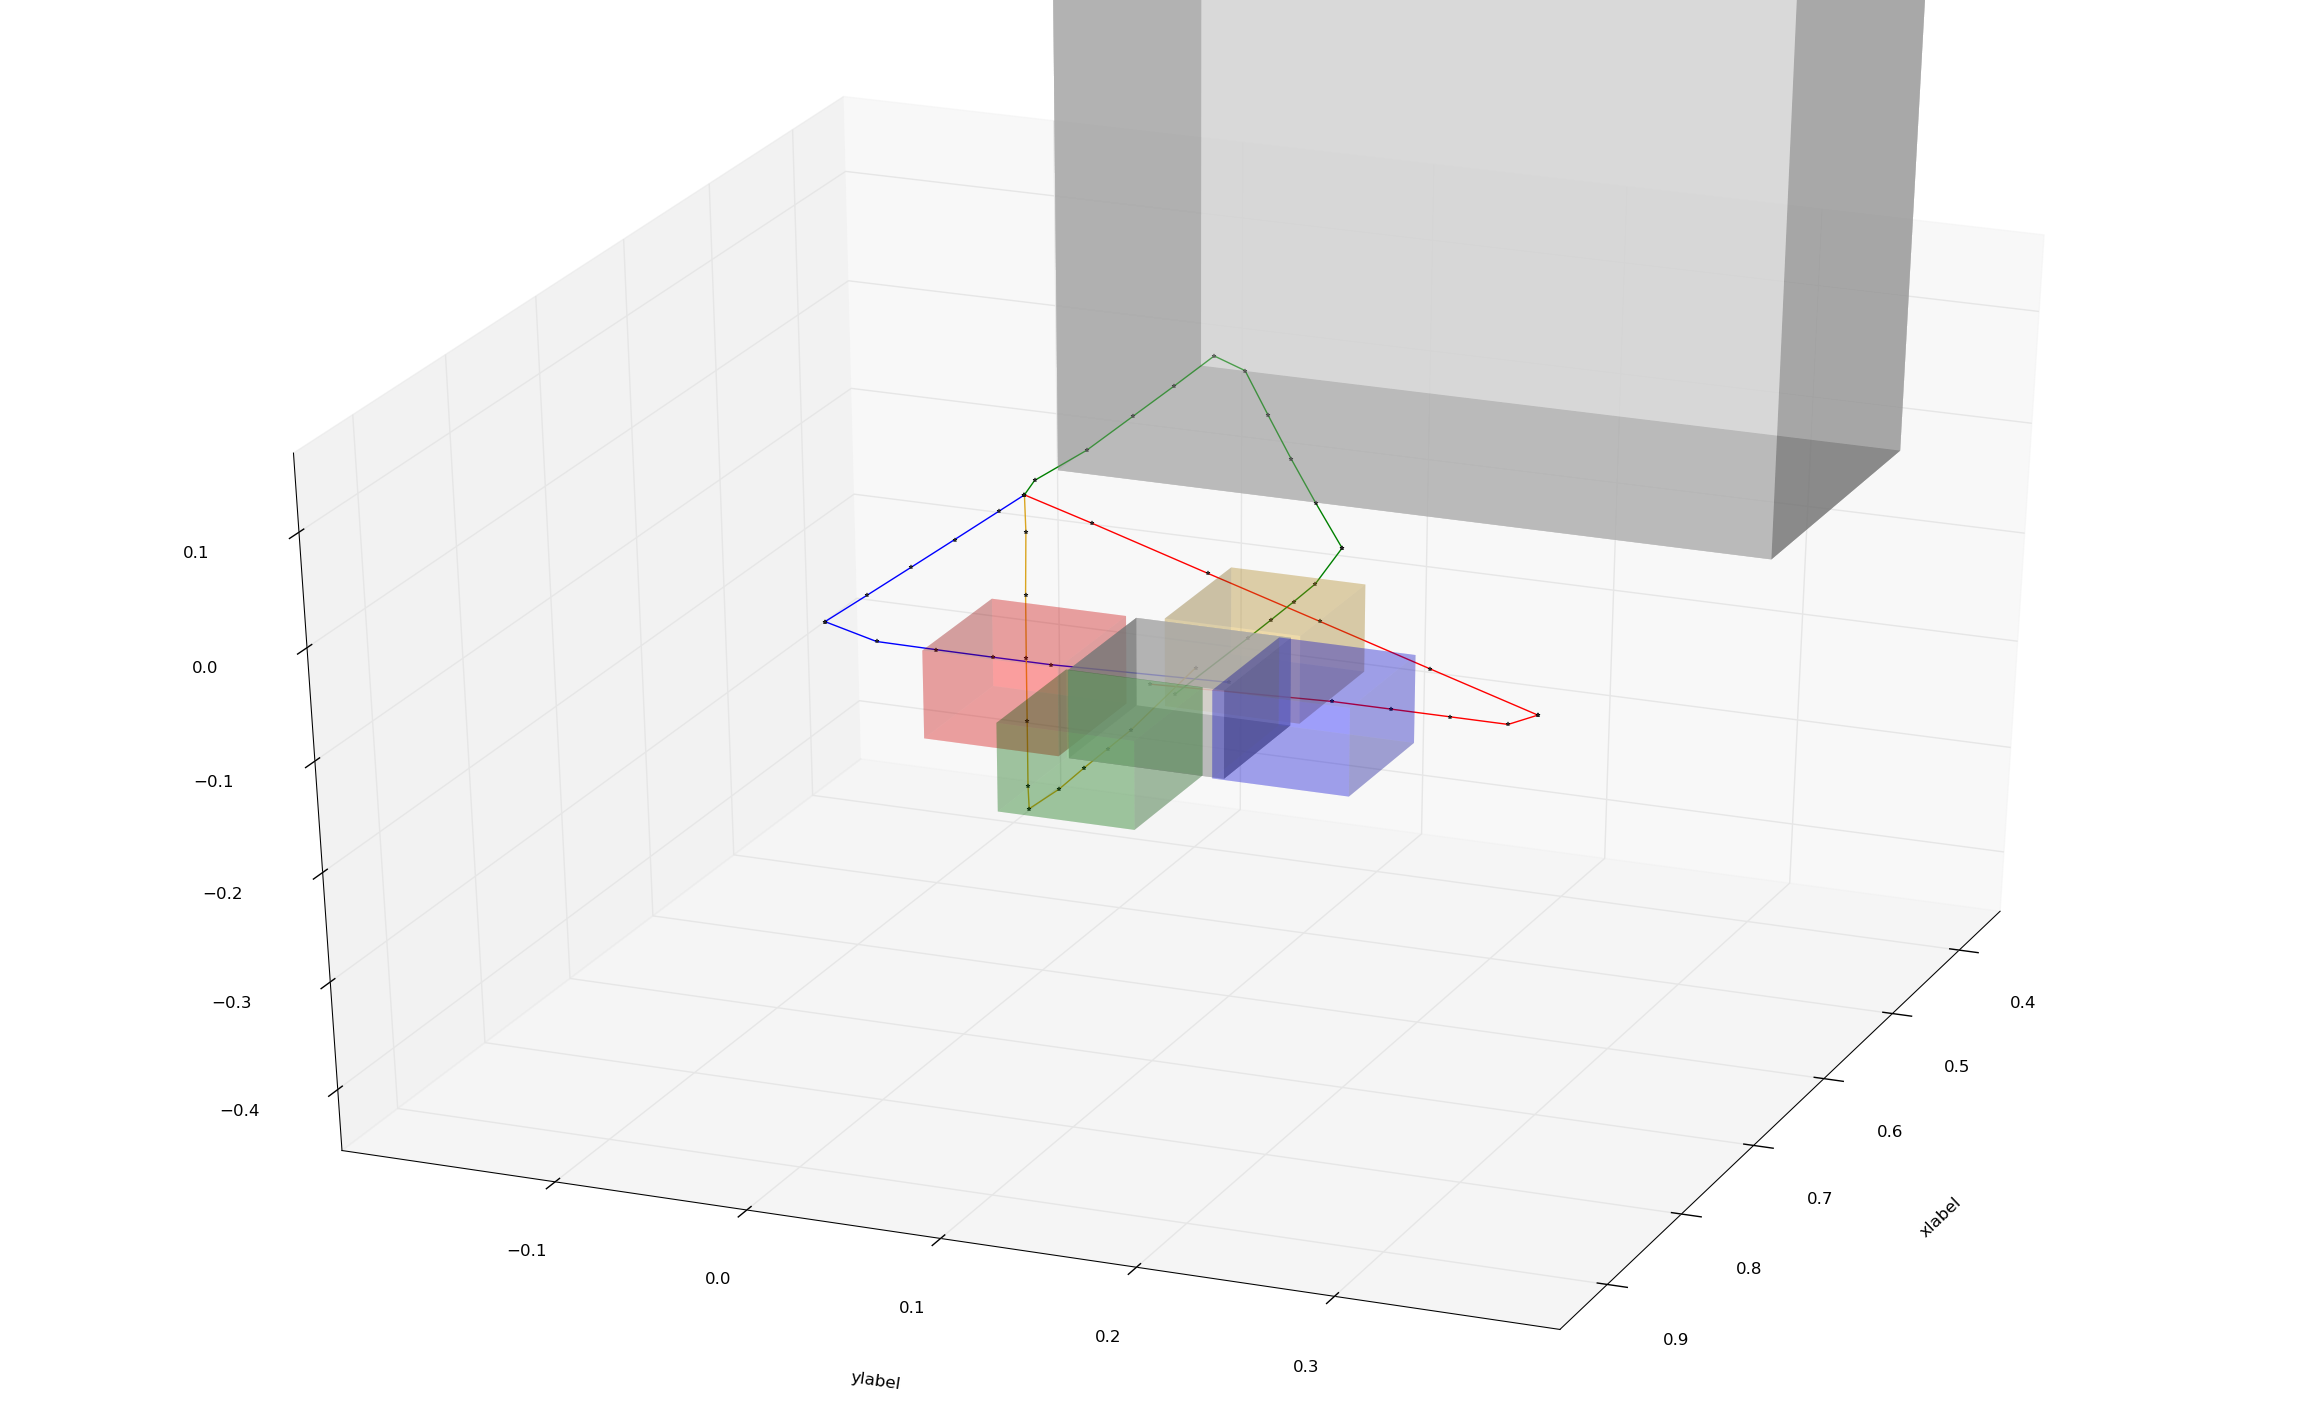
\includegraphics[width=0.9\textwidth]{figures/trajectories}
  \end{center}
  \caption{Différentes trajectoires réalisées par le robot (représenté par le volume gris). La position initiale de l'objet est représentée par le cube gris au milieu. Chaque cube coloré correspond au mouvement de la même couleur (par exemple, le cube rouge est la position finale du cube gris après avoir poussé par l'effecteur du robot suivant la trajectoire rouge).}
  \label{fig:trajectories}
\end{figure}

En raison de la nécessité de généraliser dans un contexte où le nombre d'actions est potentiellement différent et surtout inconnu, il n'est pas possible de laisser une telle valeur arbitraire.
Pour pallier à ce problème, il est nécessaire de procéder à une discrétisation adaptative de l'environnement, ce qui constitue le sujet principal de notre stage.
L'idée générale est de laisser le robot découvrir lui-même les différentes actions réalisables sans en spécifier le nombre.
Pour arriver à cet objectif, la méthode choisie lors de la définition du sujet est le clustering qui doit permettre de distinguer les différentes actions.




\subsubsection{Algorithmes de clustering}

En nous basant sur la littérature existante (\cite{Xu2015}, \cite{Andreopoulos2009}, \cite{Fahad2014} et \cite{Sajana2016}), nous avons réalisé en début de stage une synthèse des algorithmes de clustering les plus communément utilisés.
La production scientifique est riche et il existe aujourd'hui plus d'une centaine d'algorithmes de clustering, groupés en différentes catégories (voir section 4.6).
Afin de filtrer et sélectionner les algorithmes les plus pertinents pour le problème posé dans notre stage, nous avons choisi plusieurs critères non arbitraires.
En se référant à la généralisation indispensable mentionnée ci-dessus, un premier critère concerne la nécessité de ne pas fournir le nombre attendu de clusters en paramètre.
En effet, le système doit pouvoir de trouver de façon autonome un nombre d'actions permettant une clusterisation efficace.
Un second critère concerne la possibilité de travailler avec de nombreuses dimensions.
Au départ, seules deux dimensions sont prises en compte, les coordonnées $x$ et $y$.
Cependant, une évolution envisagée dès le départ concerne l'ajout de nouvelles dimensions pour la clusterisation telles que les trois dimensions concernant la rotation de l'objet.
Le troisième et dernier critère concerne la disponibilité d'une implémentation en Python ou C{}\verb!++!.
En effet, l'objectif du stage n'était pas d'implémenter un algorithme en particulier mais de réutiliser facilement des implémentations déjà existantes.
Les algorithmes ne satisfaisant pas à ces critères ont été rejetés.

Sur la centaine d'algorithmes de clustering existants, sept ont été retenus lors de cette première phase : X-means\textsuperscript{1}, Affinity Propagation\textsuperscript{1}, DBSCAN\textsuperscript{2}, HDBSCAN\textsuperscript{2}, OPTICS\textsuperscript{2}, Mean-Shift\textsuperscript{2} et Level Set Tree. (1) correspondent à des algorithmes de partitionnement et (2) correspondent à des algorithmes basés sur la densité.

% Based on \cite{Xu2015}, \cite{Andreopoulos2009}, \cite{Fahad2014} and \cite{Sajana2016}, we reviewed the most common algorithms used for clustering, grouped in categories (see annex for details). Non-arbitrary criteria were required for filtering algorithms. According to the generalization mentioned above, a first criterion concerns the requirement to pass the number of clusters as input parameter. Indeed, as the system should be able to find itself the correct number of actions. A second criterion concern the possibility to work with high dimensionality and a third one is the implemenation's availabily in Python or C++. Algorithms that did not suit to those parameters were discarded.

% The intuition behind that choice is based on the fact that the different categories of actions have roughly the same end position. In other terms, a \textbf{Left} action will end in the specific area for left actions. Hence, a large amount of space will be empty and will not contain any end positions. The points distribution would lead to focus on finding areas of high density. For that purpose, density-based algorithms exist.

% Afin de comparer les différents algorithmes, une série de tests a été réalisée avec 2 jeux de données différents : un dataset avec une distribution uniforme de points et un jeu de données généré en simulation.


% \begin{figure}
% 	\centering
% 	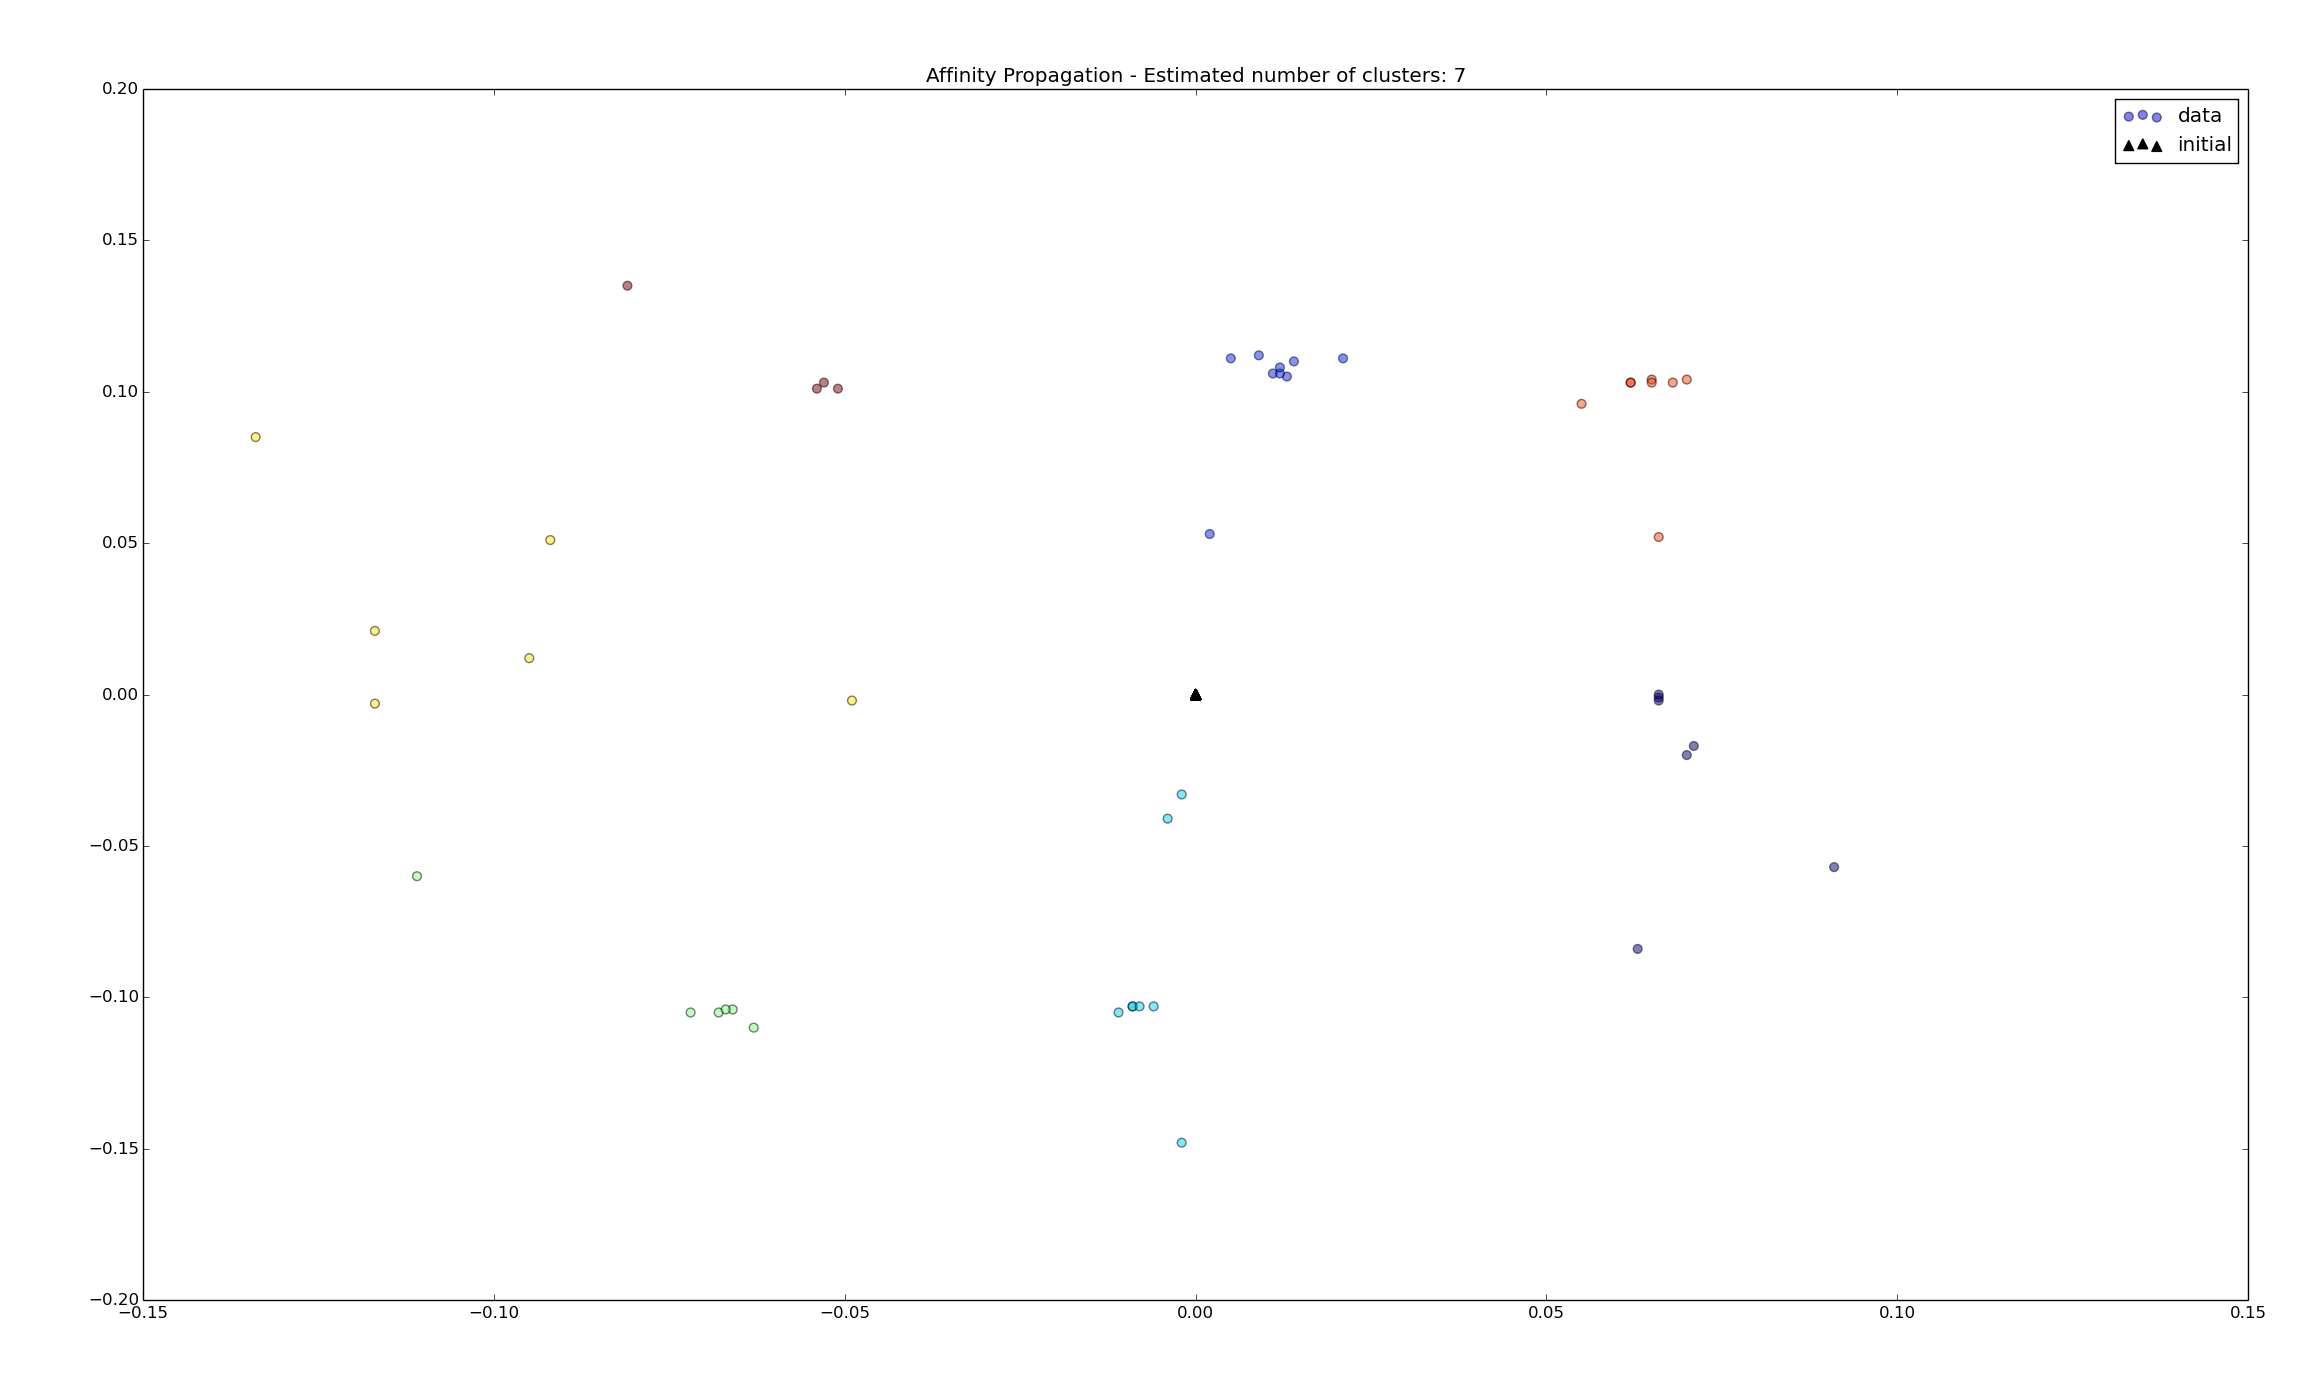
\includegraphics[width=\textwidth]{figures/clustering_results/AP}
% 	\caption{Clustering with Affinity Propagation. AP clusters correctly the dataset. Parameters are: \textit{damping=0.5, preference=-0.0095}}
% 	\label{fig:ap}
% \end{figure}



\subsubsection{Intuition}

L'enjeu consistait à trouver le meilleur algorithme de clustering et les meilleurs paramètres associés pour un jeu de données fourni.
Pour cela, notre intuition a été de réfléchir à une manière d'optimiser les paramètres des différents algorithmes jusqu'à obtenir une convergence vers un ensemble de paramètres optimaux relativement aux contraintes fournies en entrée.
Les algorithmes génétiques sont par nature efficaces pour obtenir des résultats bons à défaut d'être exacts.
Plusieurs critères étant à optimiser, nous avons donc fait le choix d'un algorithme génétique multi-objectifs.


\subsubsection{Implémentation}

Pour implémenter notre algorithme, nous avons utilisé le framework C{}\verb!++! open source Sferes \cite{Mouret2010} développé au sein de l'équipe AMAC et dédié à l'optimisation évolutionniste.
Ce framework a pour avantages d'être léger, multi-coeur et facilement extensible.
Sa rapidité est comparable à celle de codes dédiés.
De nombreux algorithmes de l'état de l'art y sont inclus (par exemple CMA-ES ou NSGA-II).
La mise en place est rapide dans la mesure où il ne reste qu'à rédiger le code de la fonction coût pour obtenir un algorithme évolutionnaire complet.


% Un très grand nombre d'algorithmes de clustering existent et ont été trouvés dans l'étape précédente.
% Sept d'entre eux ont été sélectionnés (principalement des algorithmes de partitionnemente et densité).
La méthode proposée consiste en un algorithme itératif au sein duquel un algorithme de clustering est réglé afin de satisfaire à 3 objectifs : \circled{1} le nombre de mouvements pour atteindre la cible, devant être minimisé pour faire en sorte que le robot soit le plus rapide possible, \circled{2} le nombre de clusters, devant être minimisé pour simplifier le calcul et \circled{3} la distance finale, à minimiser pour la précision du contrôle.
Dans la mesure où plusieurs objectifs sont à minimiser, nous avons sélectionné l'algorithme génétique NSGA-II\cite{Deb:2002:FEM:2221359.2221582} pour remplir cette tâche.

L'agorithme ci-dessous est utilisé par la fonction coût au sein de l'algorithme génétique NSGA-II :

% \begin{wrapfigure}{L}{0.5\textwidth}
    % \begin{minipage}{0.5\textwidth}
      \begin{algorithm}[H]
      \caption{Evaluation algorithm for fitness function}\label{euclid}
        \begin{algorithmic}[1]
          \State $E$ = \{C\textsubscript{e1}, \dots, C\textsubscript{en}\} \Comment{Set of clusters containing effects}
          \State $F$ = \{f\textsubscript{1}, \dots, f\textsubscript{n}\} \Comment{Set of final points}
          \State $I$ = (0;0) \Comment{Initial point}
          \State $t$ = 0 \Comment{Number of tries}
          \State Compute the set of effects $E$ from genotype
            \ForAll{final point $f\textsubscript{i}$ in $F$}
              \For{$j=1$ to \textit{nb\_repeat} }
                \While{$dist(I,\:f\textsubscript{i}) > \varepsilon$ \textbf{and} $t<t_{max}$}
                  \State $M = \{ m\textsubscript{i}\:|\:m\textsubscript{i} = rand(C\textsubscript{ei})\:\forall\:C\textsubscript{ei}\:\in E\}$
                  \State $m = \operatornamewithlimits{argmin}\limits_{m_i \in M}(dist(I+m\textsubscript{i},\:f\textsubscript{i}))$
                  \State Apply movement $m$ to $I$
                  \State $t = t + 1$
                \EndWhile
              \EndFor
            \EndFor
            \State return (nb clusters, \textoverline{nb movements}, \textoverline{final distance})
        \end{algorithmic}
      \end{algorithm}
  % \end{minipage}
% \end{wrapfigure}

% Principe
Le principe de cet algorithme au sein de la fonction coût est expliqué ci-après. 
Le génotype d'un individu contient le type d'algorithme de clustering à utiliser et un ou plusieurs paramètres associés à cet algorithme (générés par l'algorithme NSGA-II).
Ces paramètres permettent de constituer un clustering où les clusters représentent des ensembles d'effets.
Pour chaque point final, un processus itératif est initié dans lequel, à chaque étape, l'objectif est d'atteindre le point final.
Ce processus pour chaque point final est répété \textit{nb\_repeat} fois.
Pour cela, à chaque itération, un effet est sélectionné aléatoirement dans chaque cluster.
L'effet gardé est celui qui permet de se rapprocher le plus possible du point final.
L'itération est répétée tant que la distance entre le dernier vecteur utilisé et le point final est supérieure ou égale à \textit{epsilon} et que le nombre d'itérations ne dépasse pas une certaine limite $t_{max}$.
Enfin, le nombre de clusters générés avec les paramètres d'entrée ainsi que les valeurs moyennes du nombre de mouvements requis pour atteindre les points finaux et la distance finale sont retournés à la fin de la fonction coût.

L'algorithme de clustering \textit{X-means} ?? est un algorithme utilisé dans différents travaux de recherche sur les affordances pour clusteriser les effets ??.
Sa principale caractéristique est d'être basé sur l'algorithme \textit{K-means} et de le généraliser en tentant de déterminer automatiquement le nombre $k$ de clusters.
La validation expérimentale de notre méthode a été effectuée en utilisant l'algorithme \textit{Mean Shift} ??.
En effet, au travers de différents tests sur des jeux de données et des paramètres différents, cet algorithme se classait parmi les meilleurs.
Cet algorithme a révélé empiriquement par la suite la génération de clusters plus divers que \mbox{\textit{X-means}} lorsque ses paramètres ont été changés.
Le génotype est constitué par la valeur d'un seul paramètre décimal associé à cet algorithme.
La population initiale est constituée de 32 individus, évalués durant 25 générations. Les taux de croisement et de mutation pour NSGA-II sont respectivement de 0.8 et 0.1. Nous avons utilisé un jeu de données généré par un babillage orienté-objet simulé (voir ).
Un unique point final a été aléatoirement généré au début de l'expérience. La fonction coût a été évaluée 30 fois pour chaque individu, les valeurs moyennes des objectifs étant ensuite reportées.

Les résultats ont été comparés avec une discrétisation obtenue par une recherche de type \textit{Grid Search} dans l'espace de paramètres.
Le résultat obtenu est une succession de graphiques représentant les différents clusters obtenus avec les différentes valeurs de paramètres.
Des exemples de clusters obtenus pour différentes valeurs du paramètre \textit{quantile} de \textit{Mean Shift} sont listés dans la figure \ref{fig:validation}.

\begin{figure}[ht]
  \begin{center}
  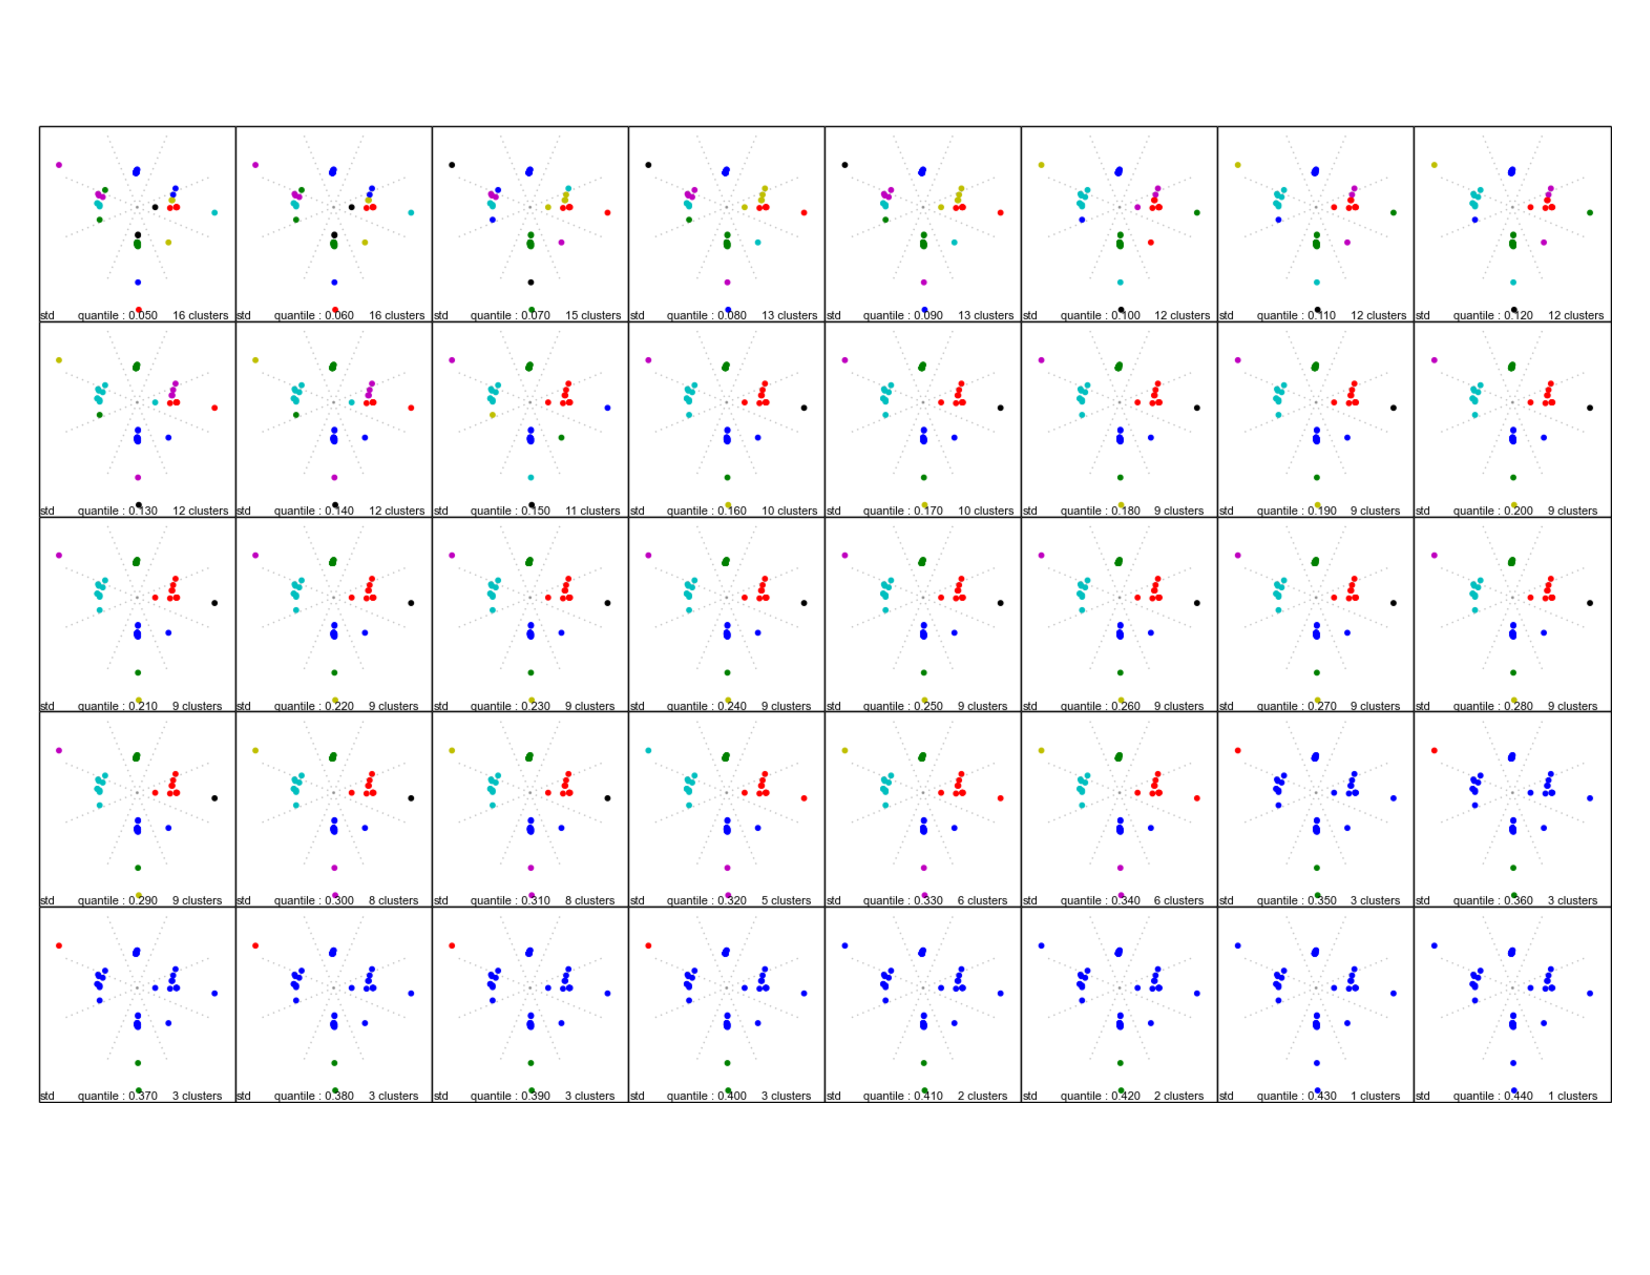
\includegraphics[width=\textwidth]{figures/DS2_MS.pdf}
    \caption{Clusters en fonction de l'évolution du paramètre \textit{quantile} de l'algorithme \textit{Mean Shift}. Les valeurs sont comprises dans l'intervalle [0.050;0.44].}
  \label{fig:validation}
  \end{center}
\end{figure}

NSGA-II étant un algorithme multi-objectif, plusieurs meilleures solutions peuvent être trouvées, correspondants aux individus dominants le front de Pareto.
La figure \ref{fig:pareto_front} montre la valeur du paramètre (de l'algorithme de clustering) correspondant aux individus dominants.
Différentes valeurs peuvent être relevées, par exemple 0.05, 0.12 ou 0.31.

À partir de cet ensemble de meilleures valeurs de paramètres, nous avons généré (voir figure \ref{fig:results}) deux séries de graphiques.
Les deux ensembles de clusters optimisent différents objectifs : vitesse et précision pour celui de gauche contre coût computationnel pour celui de droite.
La colonne de gauche contient davantage de clusters et permet un contrôle rapide et précis.
À l'inverse, l'autre solution repose sur un nombre moins important de clusters.

% \begin{figure}[!tbp]
%   \centering
%   \begin{minipage}[b]{0.4\textwidth}
%     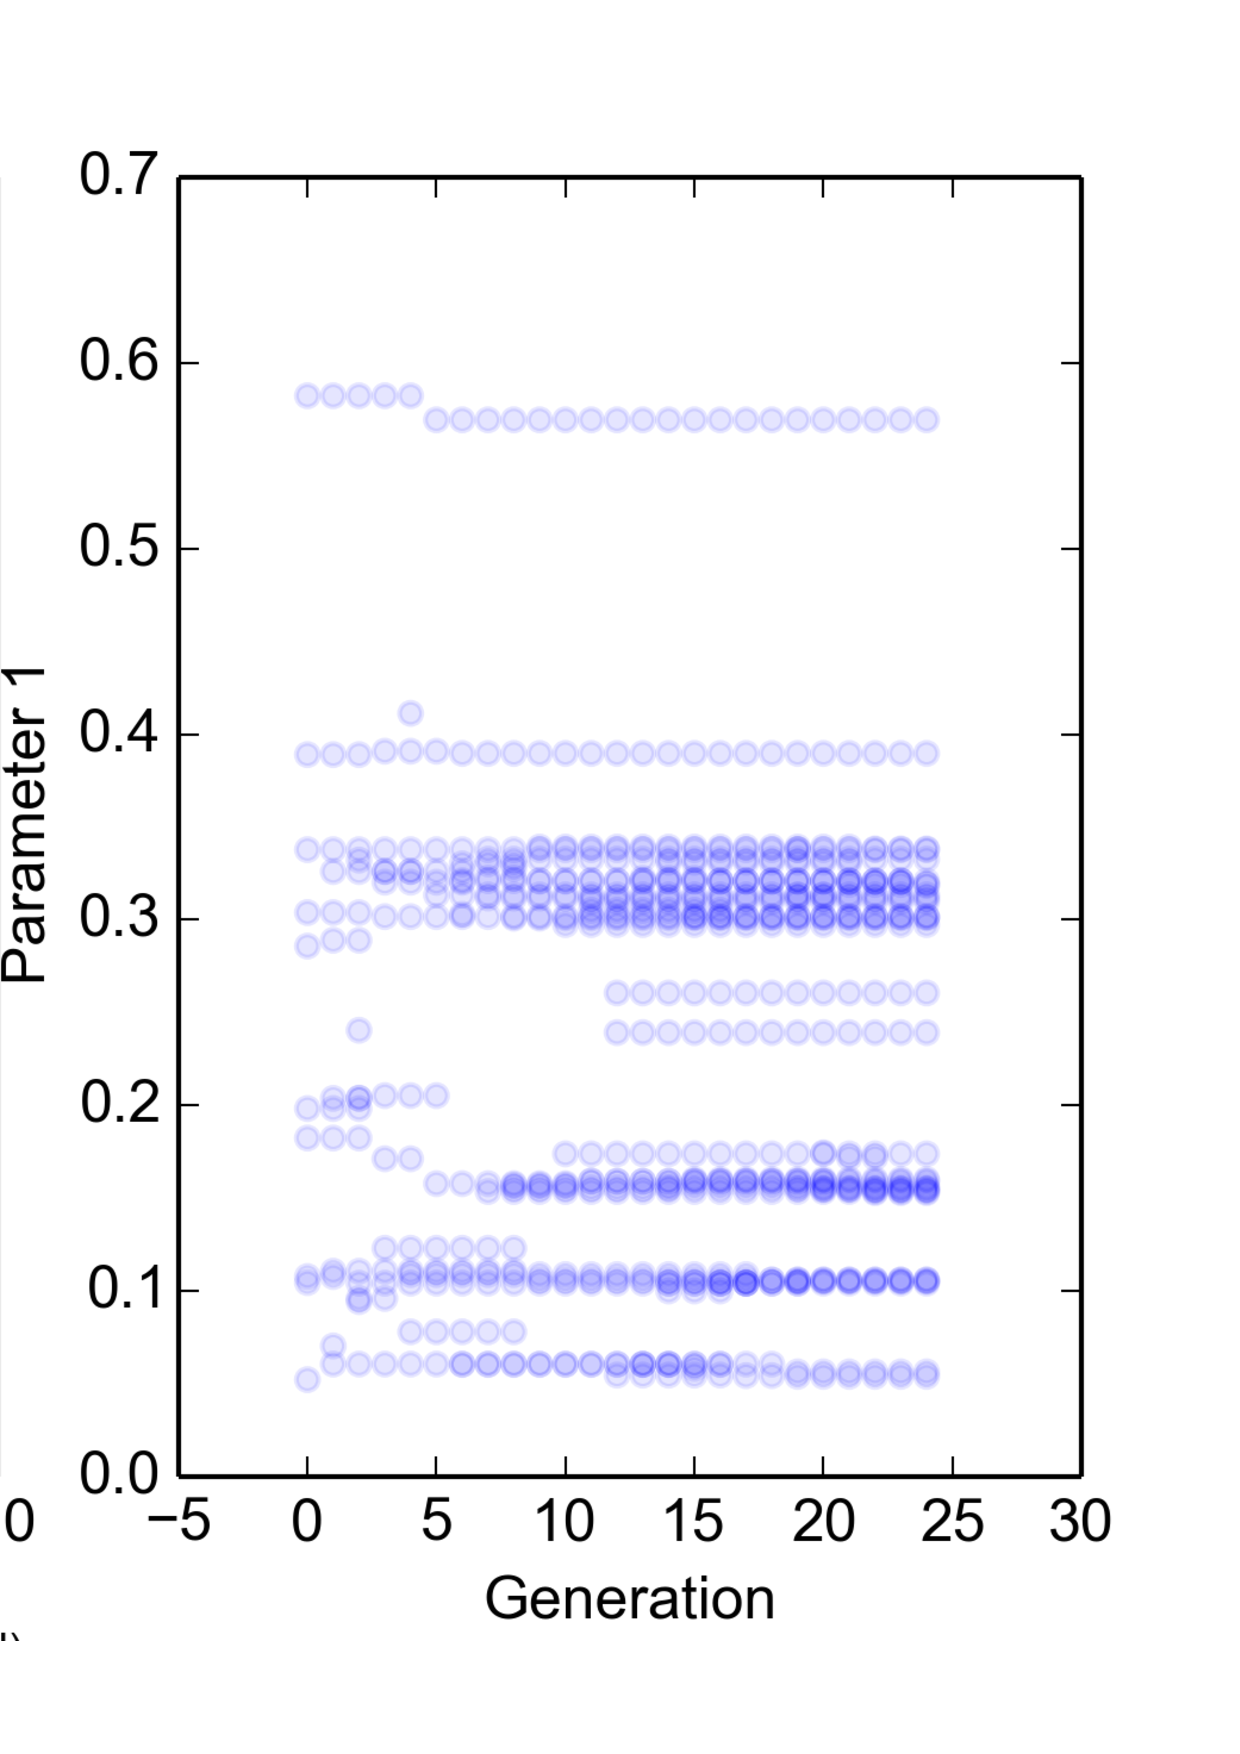
\includegraphics[width=\textwidth]{figures/Pareto_front.pdf}
%     \caption{Valeur du paramètre de l'algorithme de clustering Mean Shift correspondant aux individus dominants le front de Pareto. Plusieurs valeurs se détachent, par exemple $0.05$, $0.11$ ou $0.3$.}
%     \label{fig:pareto_front}
%   \end{minipage}
%   \hfill
%   \begin{minipage}[b]{0.5\textwidth}
%     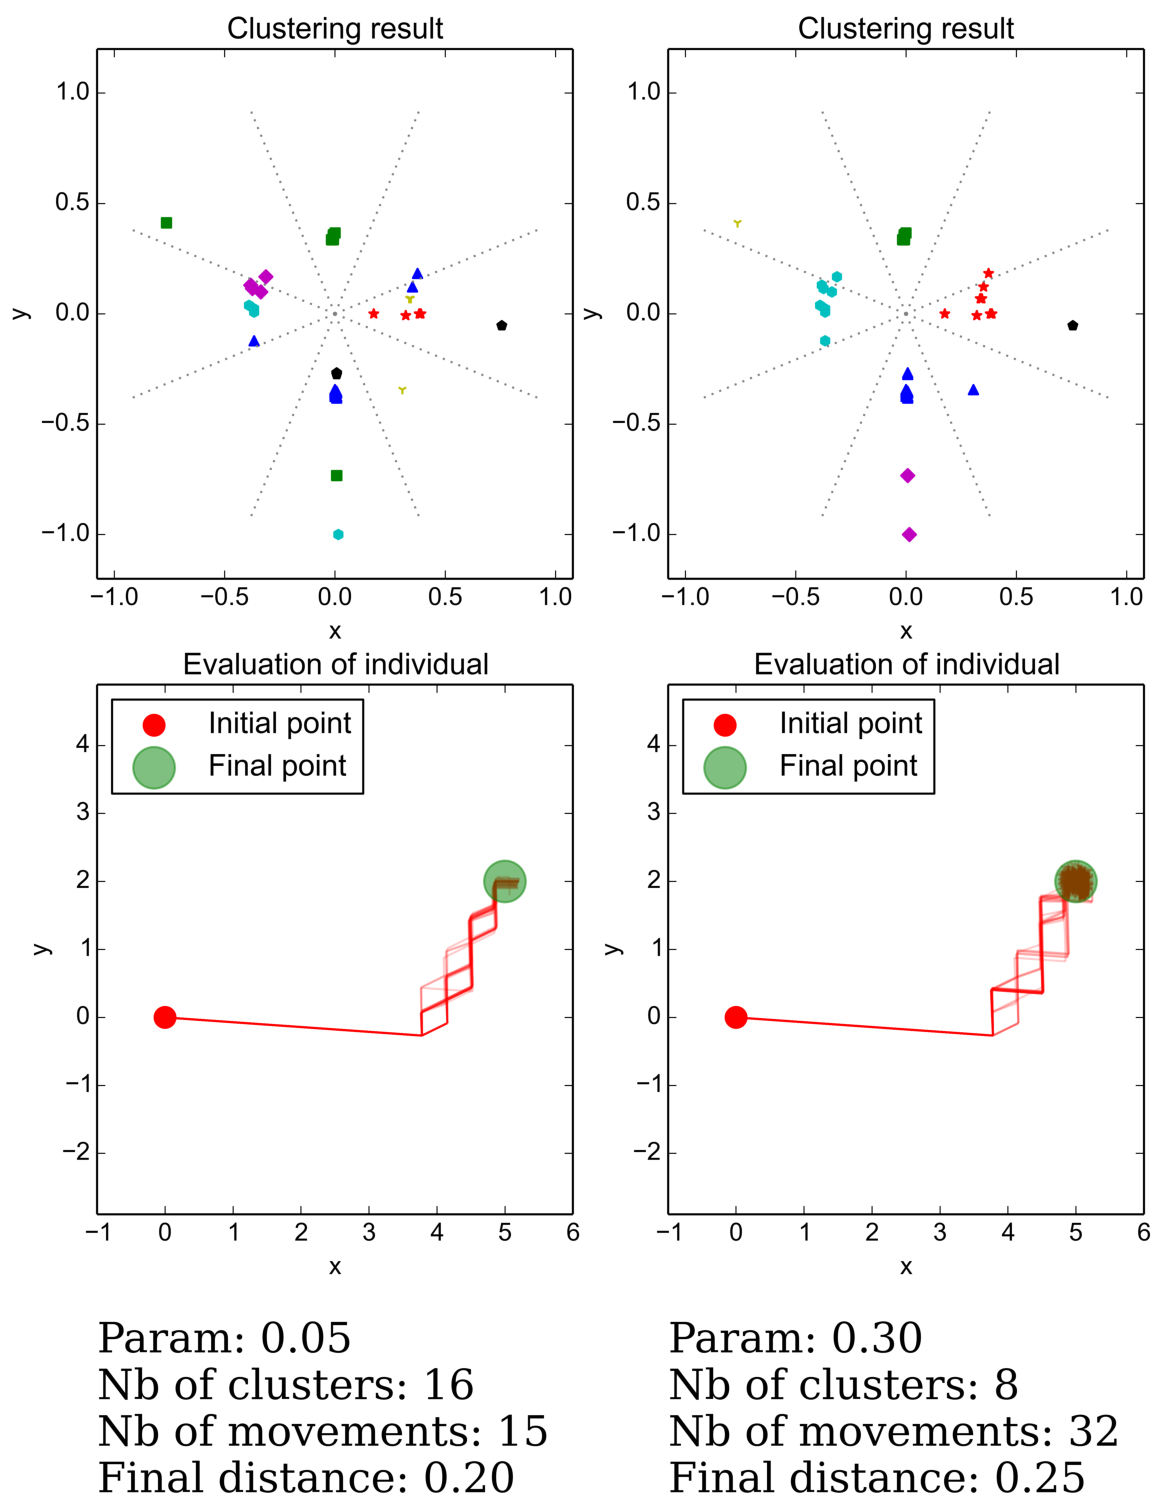
\includegraphics[width=\textwidth]{figures/Benchmark_3.pdf}
%     \caption{Les deux colonnes montrent différents résultats de clustering et de trajectoires d'évaluations basés sur les valeurs de paramètres appartenant aux individus dominants le front de Pareto.}
%     \label{fig:results}
%   \end{minipage}
% \end{figure}

\begin{figure}[ht]
  \begin{center}
    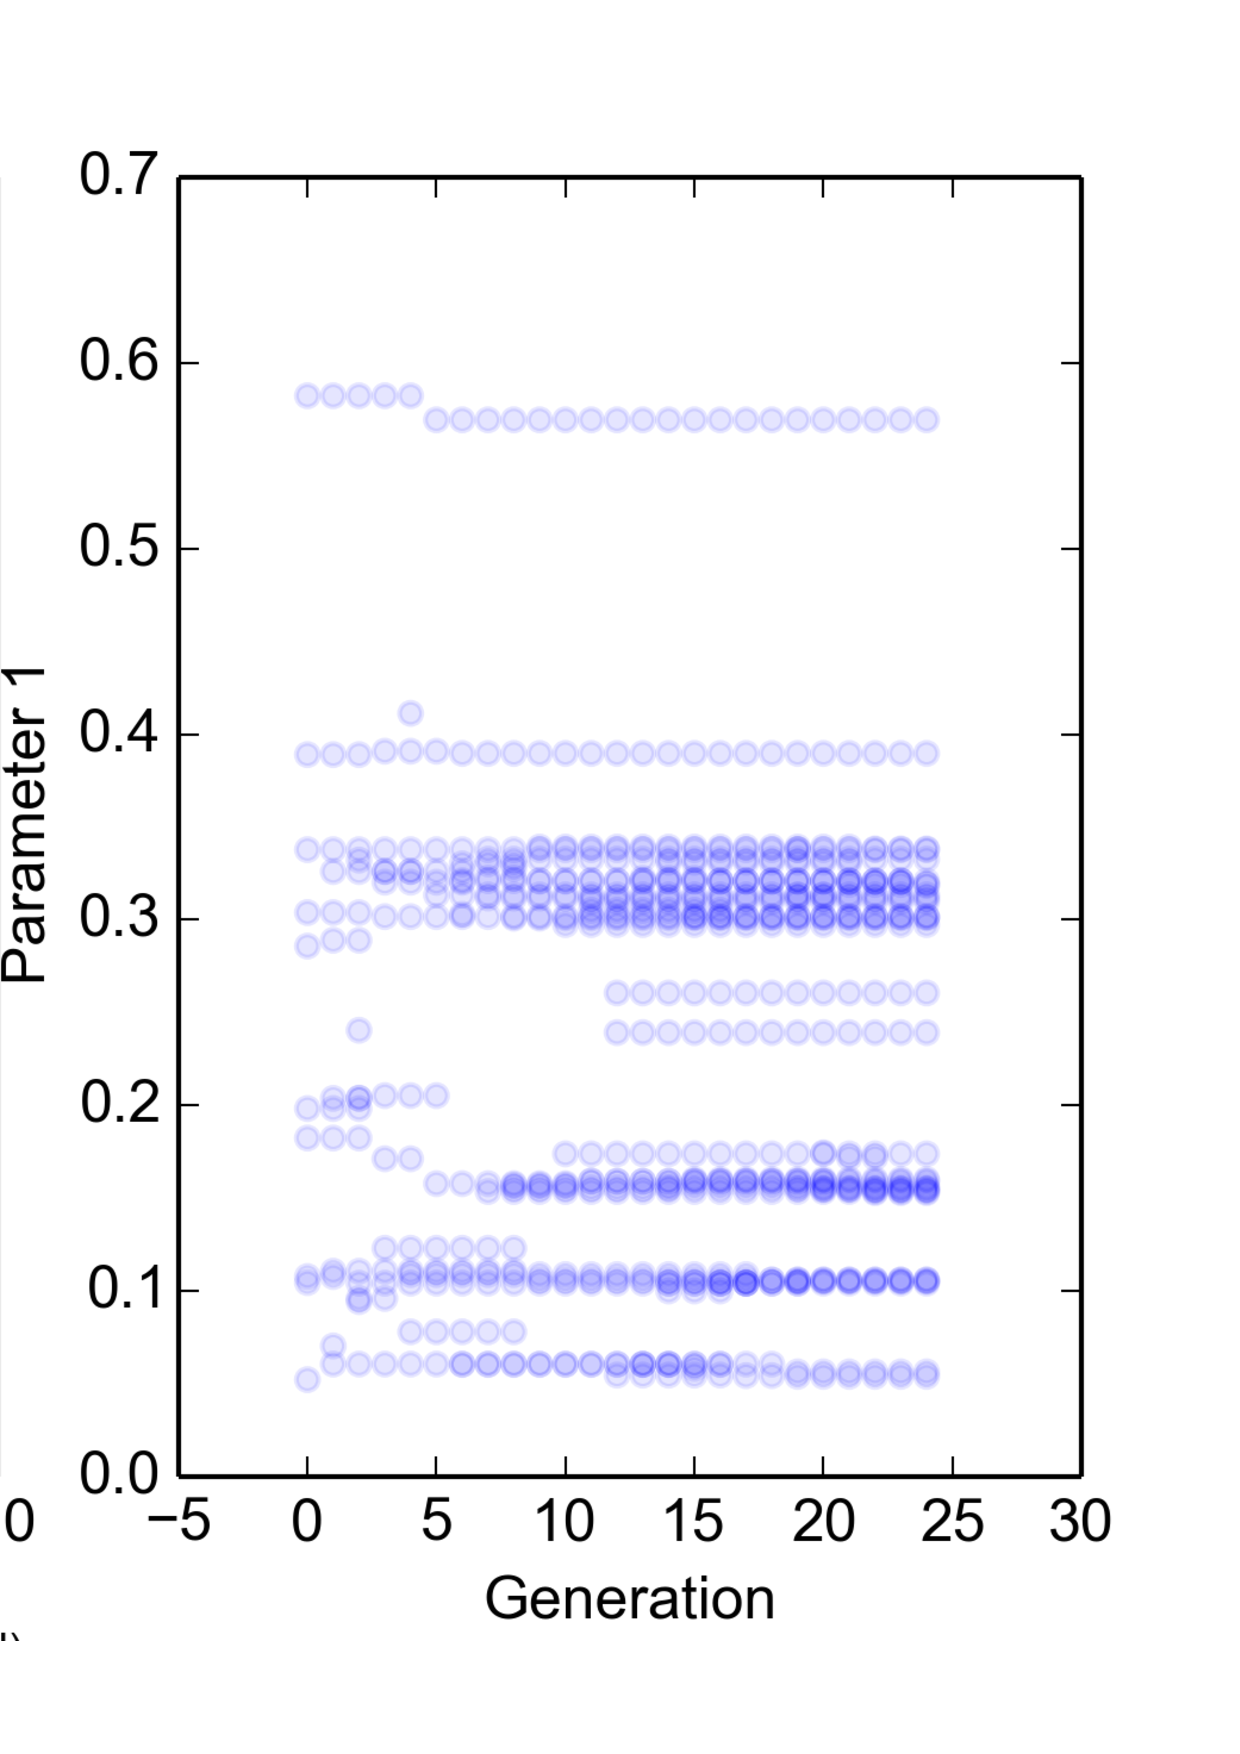
\includegraphics[width=0.5\textwidth]{figures/Pareto_front.pdf}
    \caption{Valeur du paramètre de l'algorithme de clustering Mean Shift correspondant aux individus dominants le front de Pareto. Plusieurs valeurs se détachent, par exemple $0.05$, $0.11$ ou $0.3$.}
    \label{fig:pareto_front}
  \end{center}
\end{figure}

\begin{figure}[ht]
  \begin{center}
    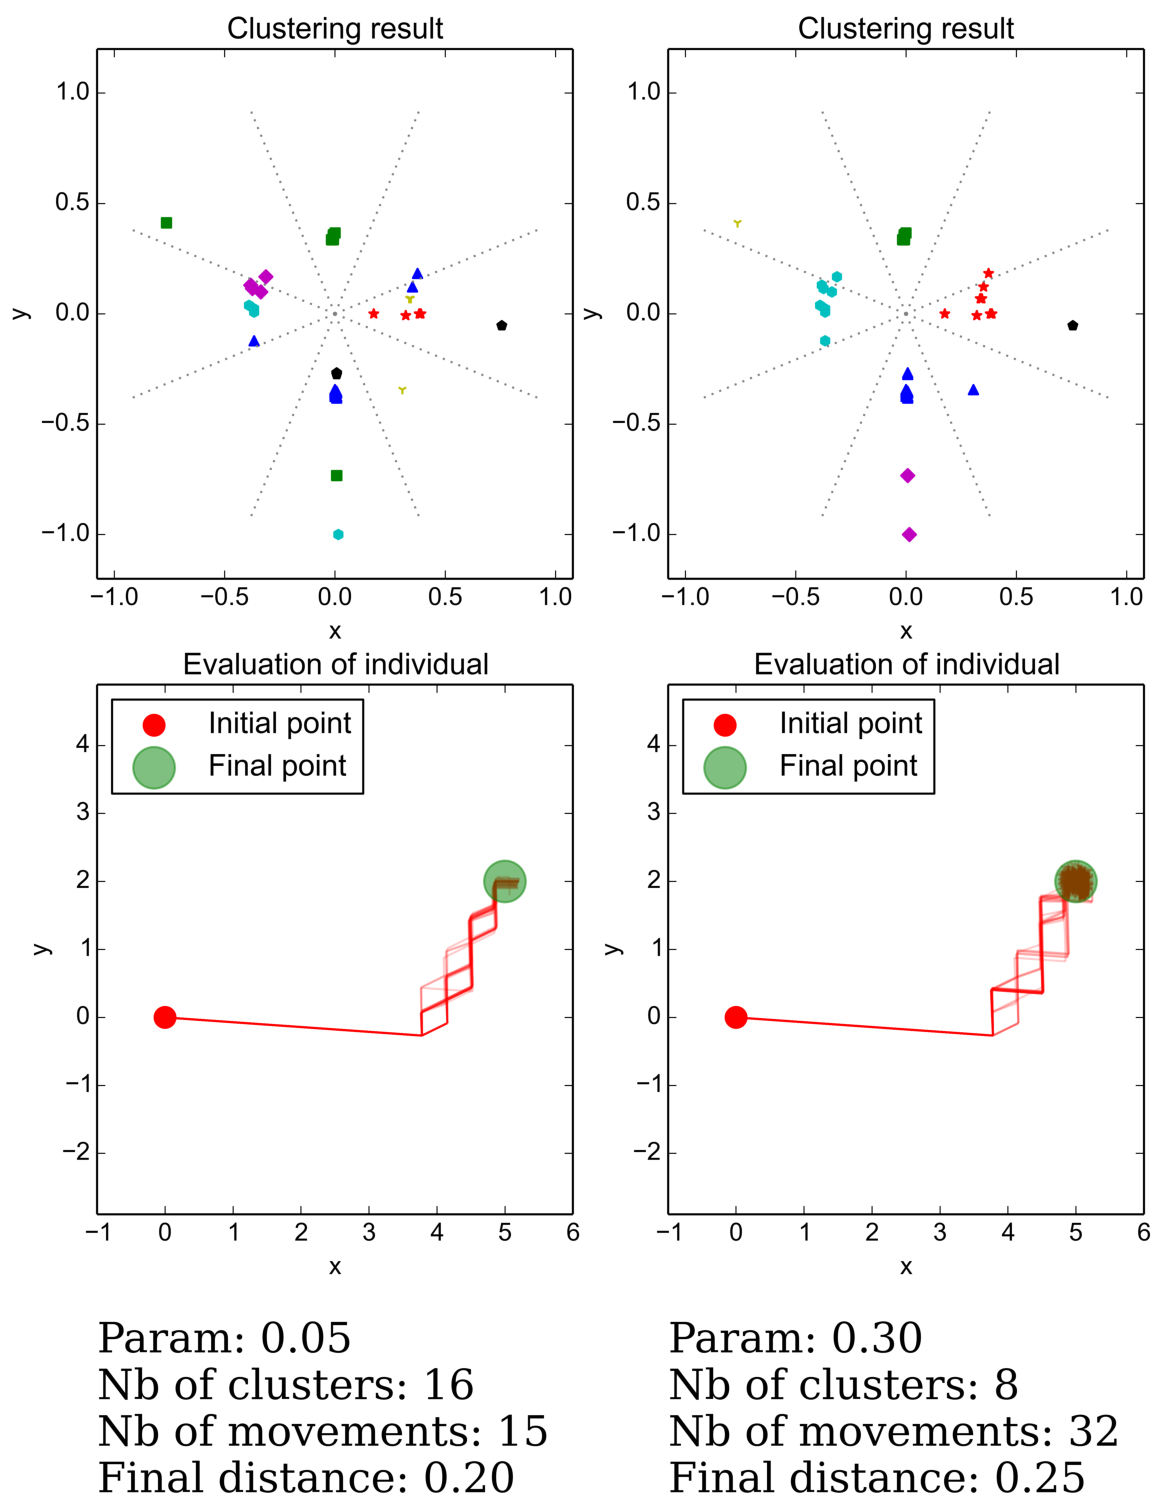
\includegraphics[width=0.6\textwidth]{figures/Benchmark_3.pdf}
    \caption{Les deux colonnes montrent différents résultats de clustering et de trajectoires d'évaluations basés sur les valeurs de paramètres appartenant aux individus dominants le front de Pareto.}
    \label{fig:results}
  \end{center}
\end{figure}


% Clusterisation based on Ugur's paper: 40 features. Compare Ugur's work with us.\\

Cette première partie de notre stage, comprenant la proposition d'un algorithme de clusterisation d'effets, a fait l'objet d'une soumission d'un abstract au workshop \textit{Developmental learning and representation building in human-robots and ambient intelligence systems} de la conférence ECAL2017\footnote{https://project.inria.fr/ecal2017/} qui se tiendra à Lyon en septembre 2017.






\subsection{Expérience de validation}

La seconde partie de notre stage a consisté à mener une expérience pour valider l'algorithme de clusterisation d'effets défini dans la première partie de ce mémoire.
Dans un premier temps, l'expérimentation s'est déroulée en simulation.
Une fois cette simulation validée (non encore réalisé à ce jour), il est prévu d'utiliser le robot afin de tester notre algorithme dans un environnement réel.

Cette expérience peut être divisée en 3 étapes : tout d'abord la génération du babillage sensorimoteur et l'enregistrement des effets pour les différents objets, puis la réalisation de la clusterisation des effets et enfin le test de l'apprentissage.
La figure \ref{fig:setup} représente la mise en place initiale de l'expérimentation.



\subsubsection{Babillage}

Durant la première étape de cette expérimentation, un objet (par exemple un cube) est placé sur la table à une position initiale.
Un babillage sur l'objet est réalisé afin d'obtenir des jeux de données contenant les différents effets découverts à traiter.
Ce babillage est effectué à l'aide de l'algorithme \textit{NovEB} (Novelty-driven Evolutionary Babbling) décrit par Maestre et al. \cite{Maestre2015}.
Cet algorithme utilise l'algorithme évolutionnaire \textit{Novelty Search} \cite{5949955} pour générer des trajectoires sans connaissance de l'environnement et des objets à priori. 
Il est capable de générer plusieurs milliers d'interactions différentes avec l'environnement, ce qui représente davantage de trajectoires qu'avec un babillage aléatoire.
Pour cela, les trajectoires sont générées en se basant sur la maximisation d'un critère de nouveauté.
Ce critère est la distance moyenne entre la trajectoire courante et ses $k$ plus proches voisins dans la population courante et dans une archive de trajectoires précédemment explorées.
Les trajectoires générées sont celles qui augmentent le plus de nouveauté.
L'algorithme NovEB génère un dataset qui peut être traité ensuite par des algorithmes de Machine Learning.
La figure \ref{fig:ns_traj} montre un exemple de trajectoire touchant l'objet considéré.

% \begin{figure}[!tbp]
%   \centering
%   \begin{minipage}[b]{0.45\textwidth}
%     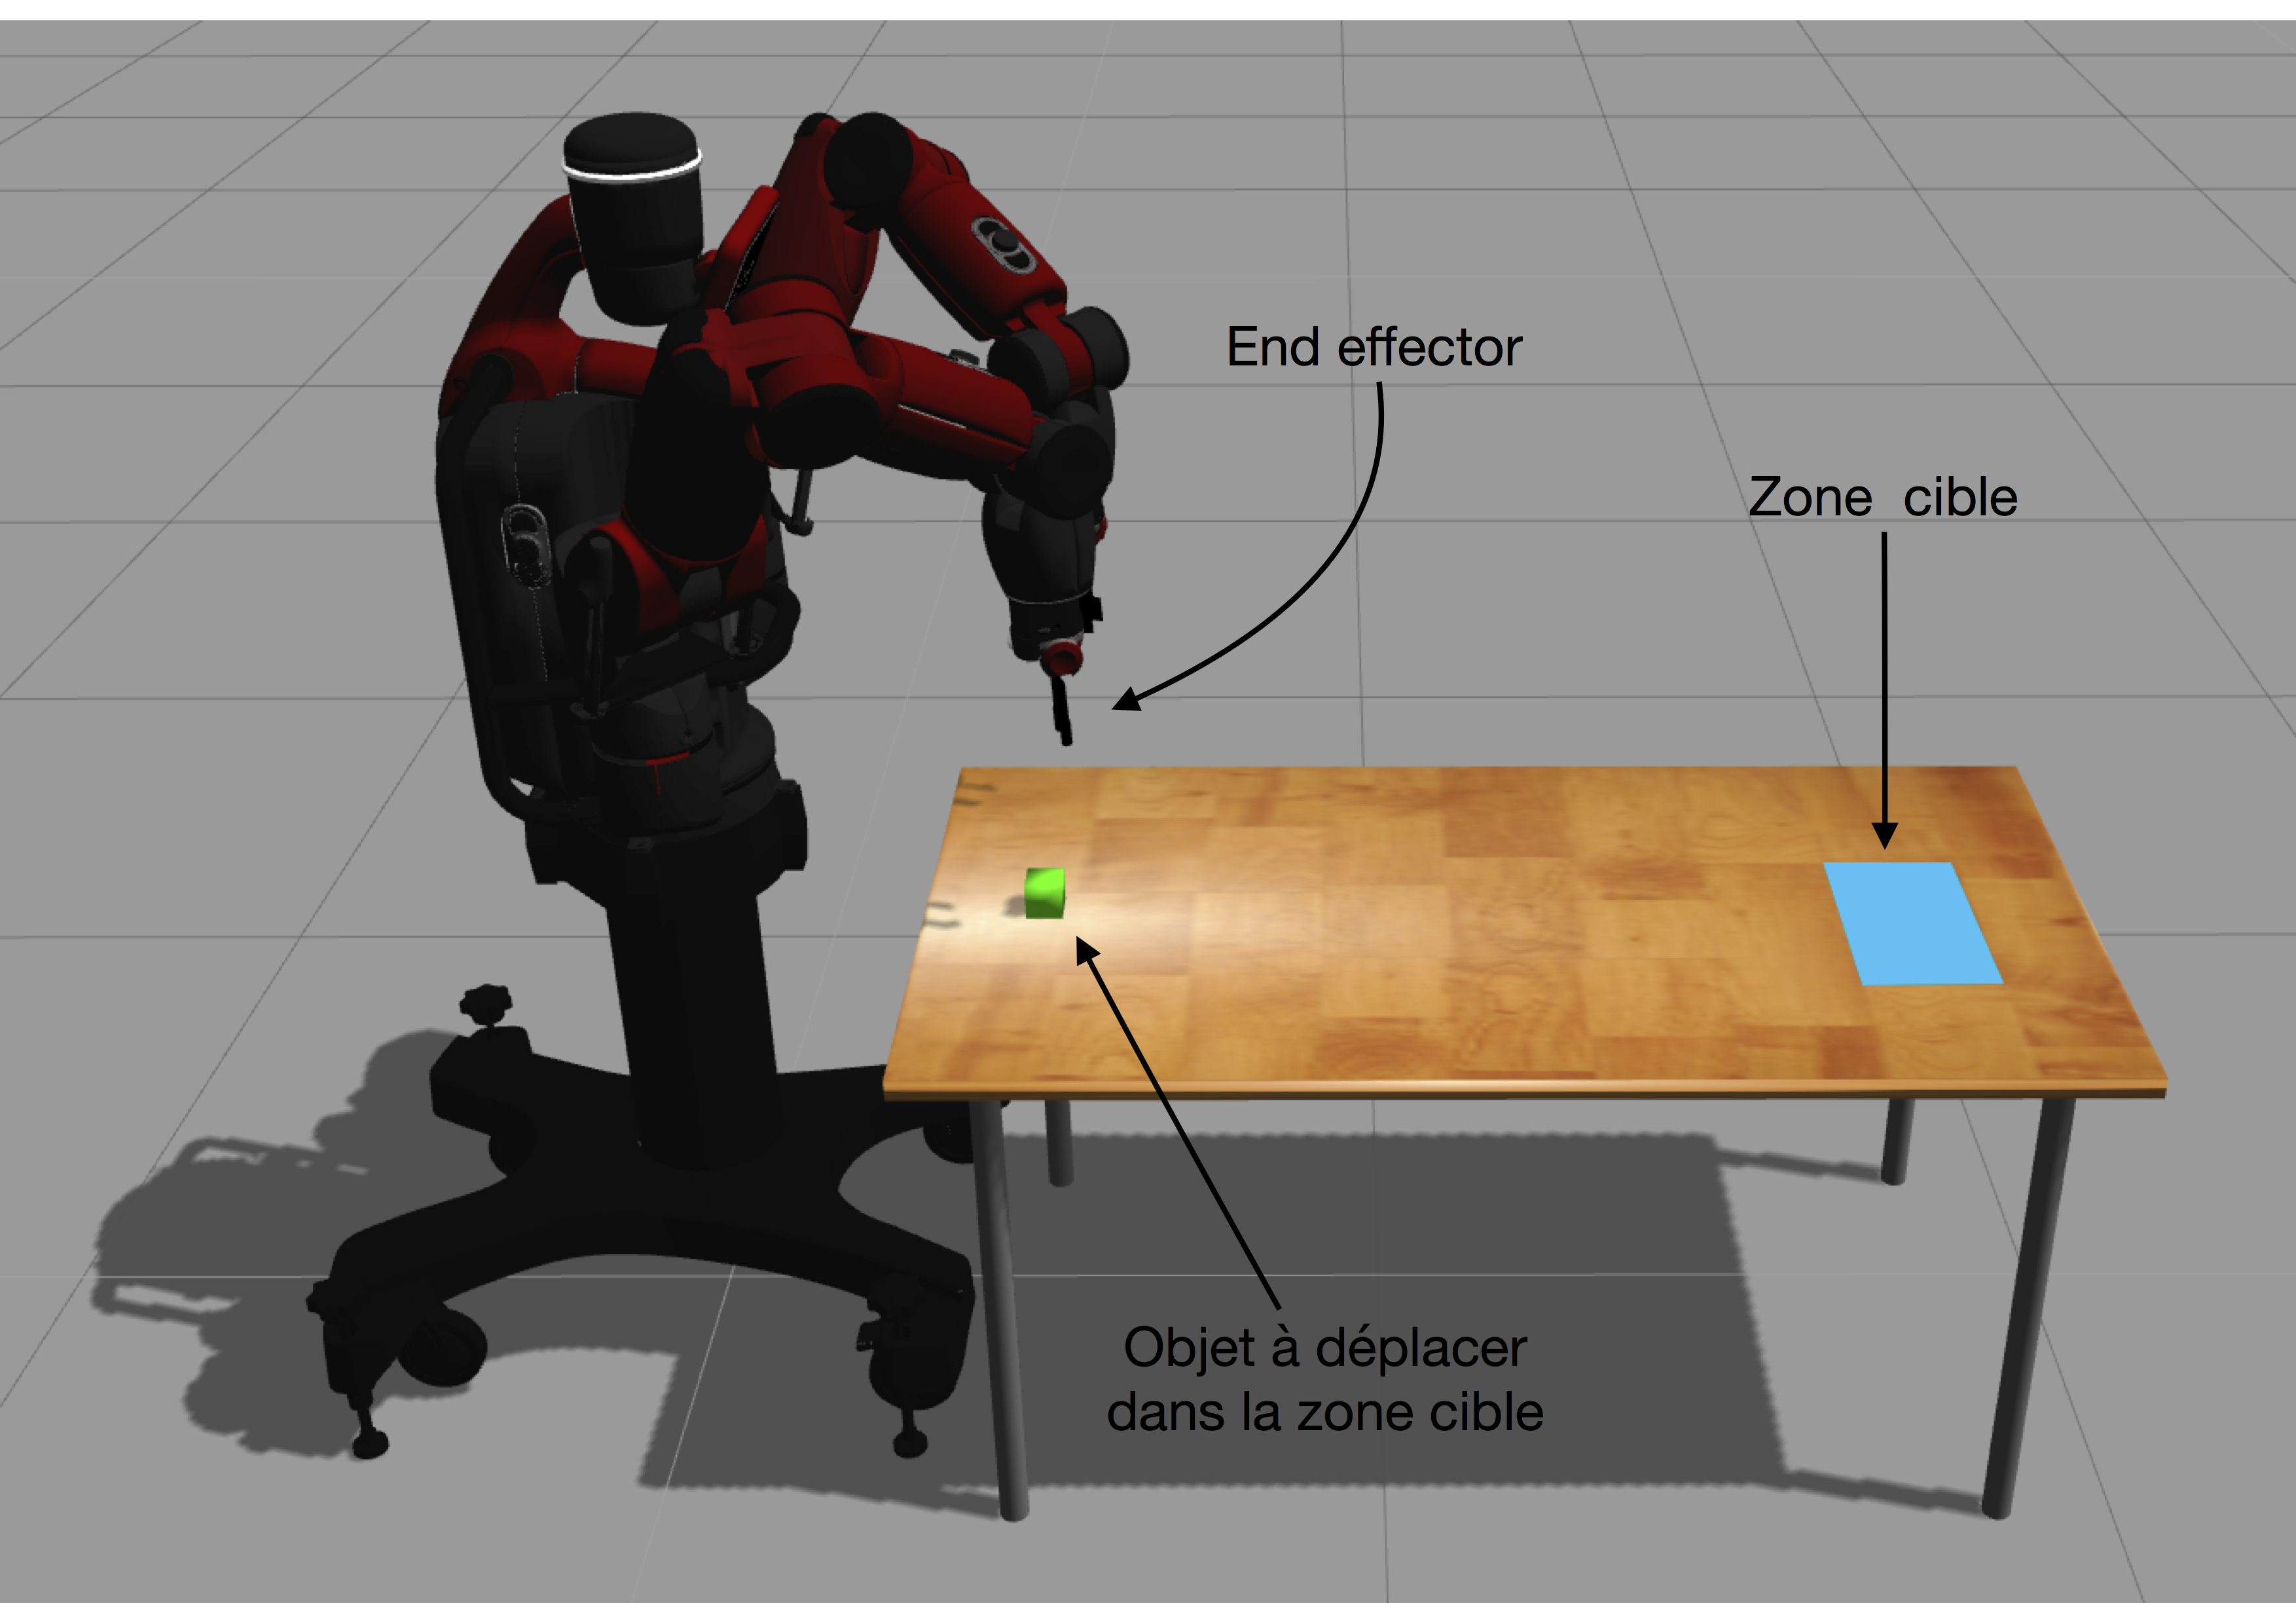
\includegraphics[width=\textwidth]{figures/Experiment_setup_annoted_FR.png}
%     \caption{L'objectif du robot est d'apprendre à pousser différents objets (par exemple, le cube vert) depuis sa position initiale jusqu'à la zone cible en bleu, en dehors de la portée du bras du robot. Une première étape de babillage permet de découvrir les effets qui sont clusterisés à l'aide de l'algorithme de clusterisation. Enfin, dans une troisième étape, le robot tente d'atteindre la zone cible.}
%     \label{fig:setup}
%   \end{minipage}
%   \hfill
%   \begin{minipage}[b]{0.45\textwidth}
%     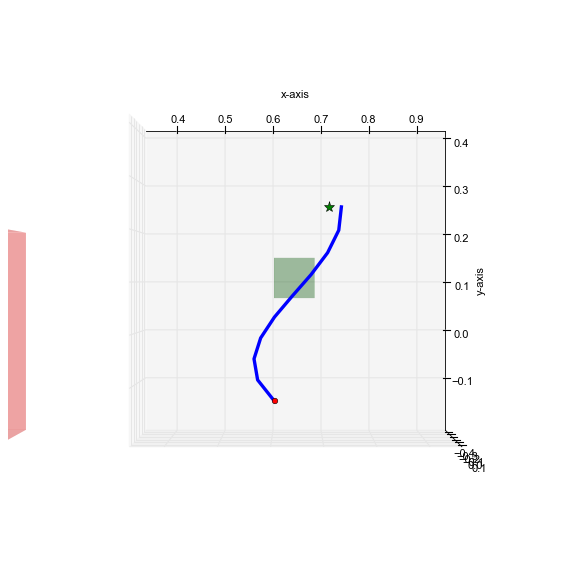
\includegraphics[width=\textwidth]{figures/ns_trajectory.png}
%     \caption{Génération de trajectoire avec NovEB. Le rectangle rouge représente l'emplacement du robot. Le point rouge correspond à la position initiale de l'effecteur du robot. Le tracé en bleu correspond à la trajectoire de cet effecteur vers l'objet. L'étoile verte indique la position de l'objet à la fin de l'exécution de la trajectoire de l'effecteur.}
%     \label{fig:ns_traj}
%   \end{minipage}
% \end{figure}

\begin{figure}[ht]
  \begin{center}
    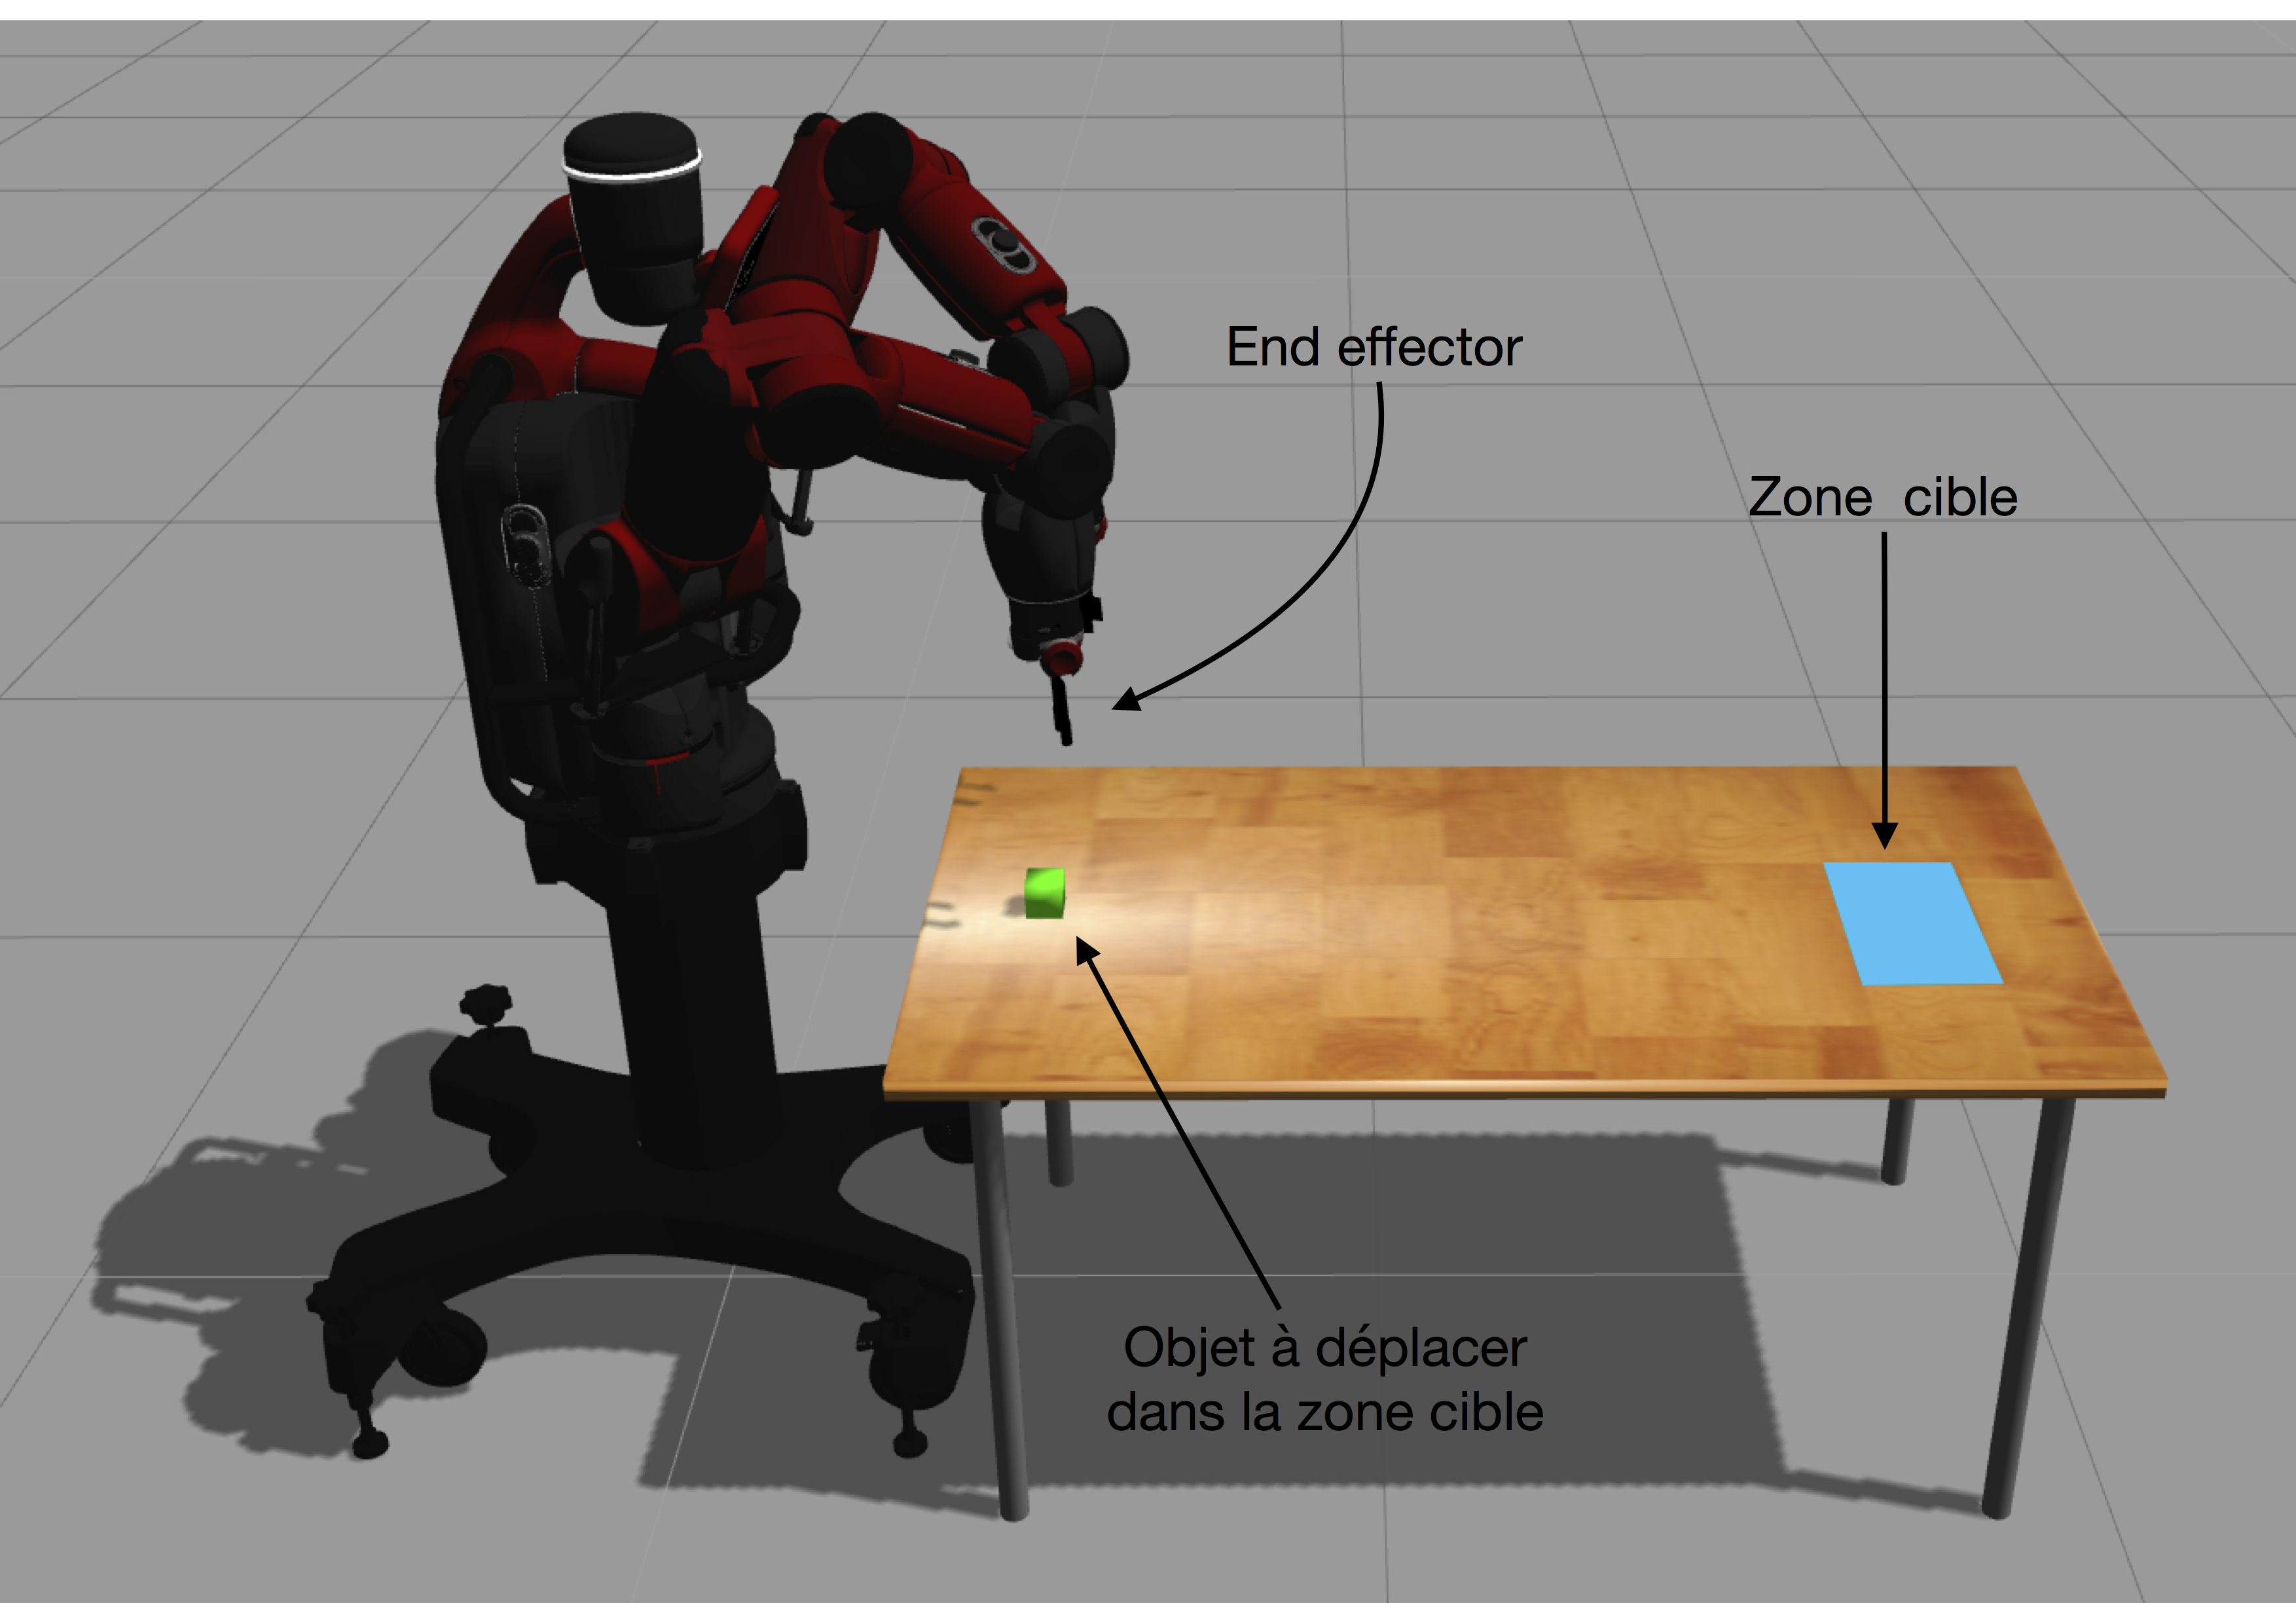
\includegraphics[width=0.6\textwidth]{figures/Experiment_setup_annoted_FR.png}
    \caption{L'objectif du robot est d'apprendre à pousser différents objets (par exemple, le cube vert) depuis sa position initiale jusqu'à la zone cible en bleu, en dehors de la portée du bras du robot. Une première étape de babillage permet de découvrir les effets qui sont clusterisés à l'aide de l'algorithme de clusterisation. Enfin, dans une troisième étape, le robot tente d'atteindre la zone cible.}
    \label{fig:setup}
  \end{center}
\end{figure}

\begin{figure}[ht]
  \begin{center}
    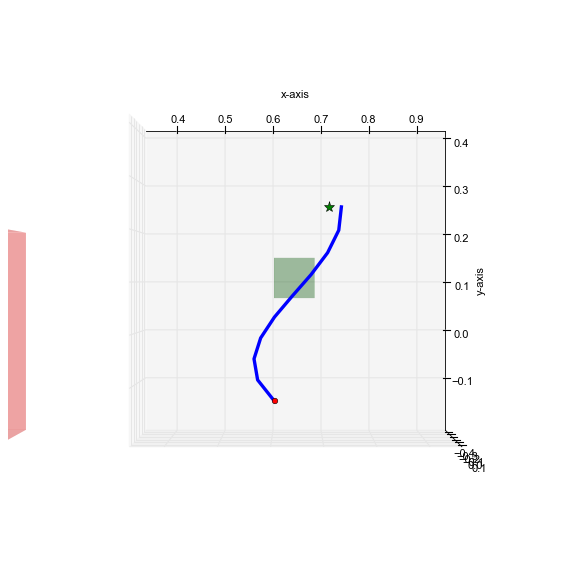
\includegraphics[width=0.6\textwidth]{figures/ns_trajectory.png}
    \caption{Génération de trajectoire avec NovEB. Le rectangle rouge représente l'emplacement du robot. Le point rouge correspond à la position initiale de l'effecteur du robot. Le tracé en bleu correspond à la trajectoire de cet effecteur vers l'objet. L'étoile verte indique la position de l'objet à la fin de l'exécution de la trajectoire de l'effecteur.}
    \label{fig:ns_traj}
  \end{center}
\end{figure}




\subsubsection{Clusterisation d'effets}

La seconde étape de l'expérience de validation implique l'algorithme que nous avons présenté dans la première partie et vise à clusteriser les effets présents dans les jeux de données.
Il en résulte une variété de paramètres de l'algorithme de clusterisation considéré qui peuvent être exploités durant la troisième étape.
Les meilleurs paramètres trouvés dans l'étape précédente sont utilisés pour pousser les différents objets vers la zone cible.
Dans notre expérience, une valeur du paramètre \textit{quantile} est sélectionnée (par exemple 0.18) et utilisée pour générer le clustering utilisé par le robot.

% La première étape consiste donc en un babillage. Concrétement, la position de l'objet sur l'espace de travail est récupérée ainsi que la position de l'effecteur. Une trajectoire est ensuite générée à l'aide de la cinématique inverse et Novelty Search afin d'atteindre l'objet. Cet objet est positionné de façon aléatoire dans les intervalles [x;x] et [y;y].



\subsubsection{Test de l'apprentissage}

Enfin, dans un troisième temps, l'objectif du robot est de pousser l'objet présenté devant lui vers une zone cible (dont la position est variable), en utilisant les différents effets à sa disposition trouvés lors de l'étape précédente.
Cette dernière étape soulève plusieurs problèmes qu'il a fallu ou qu'il faut résoudre.

% \begin{figure}[ht]
%   \begin{center}
%   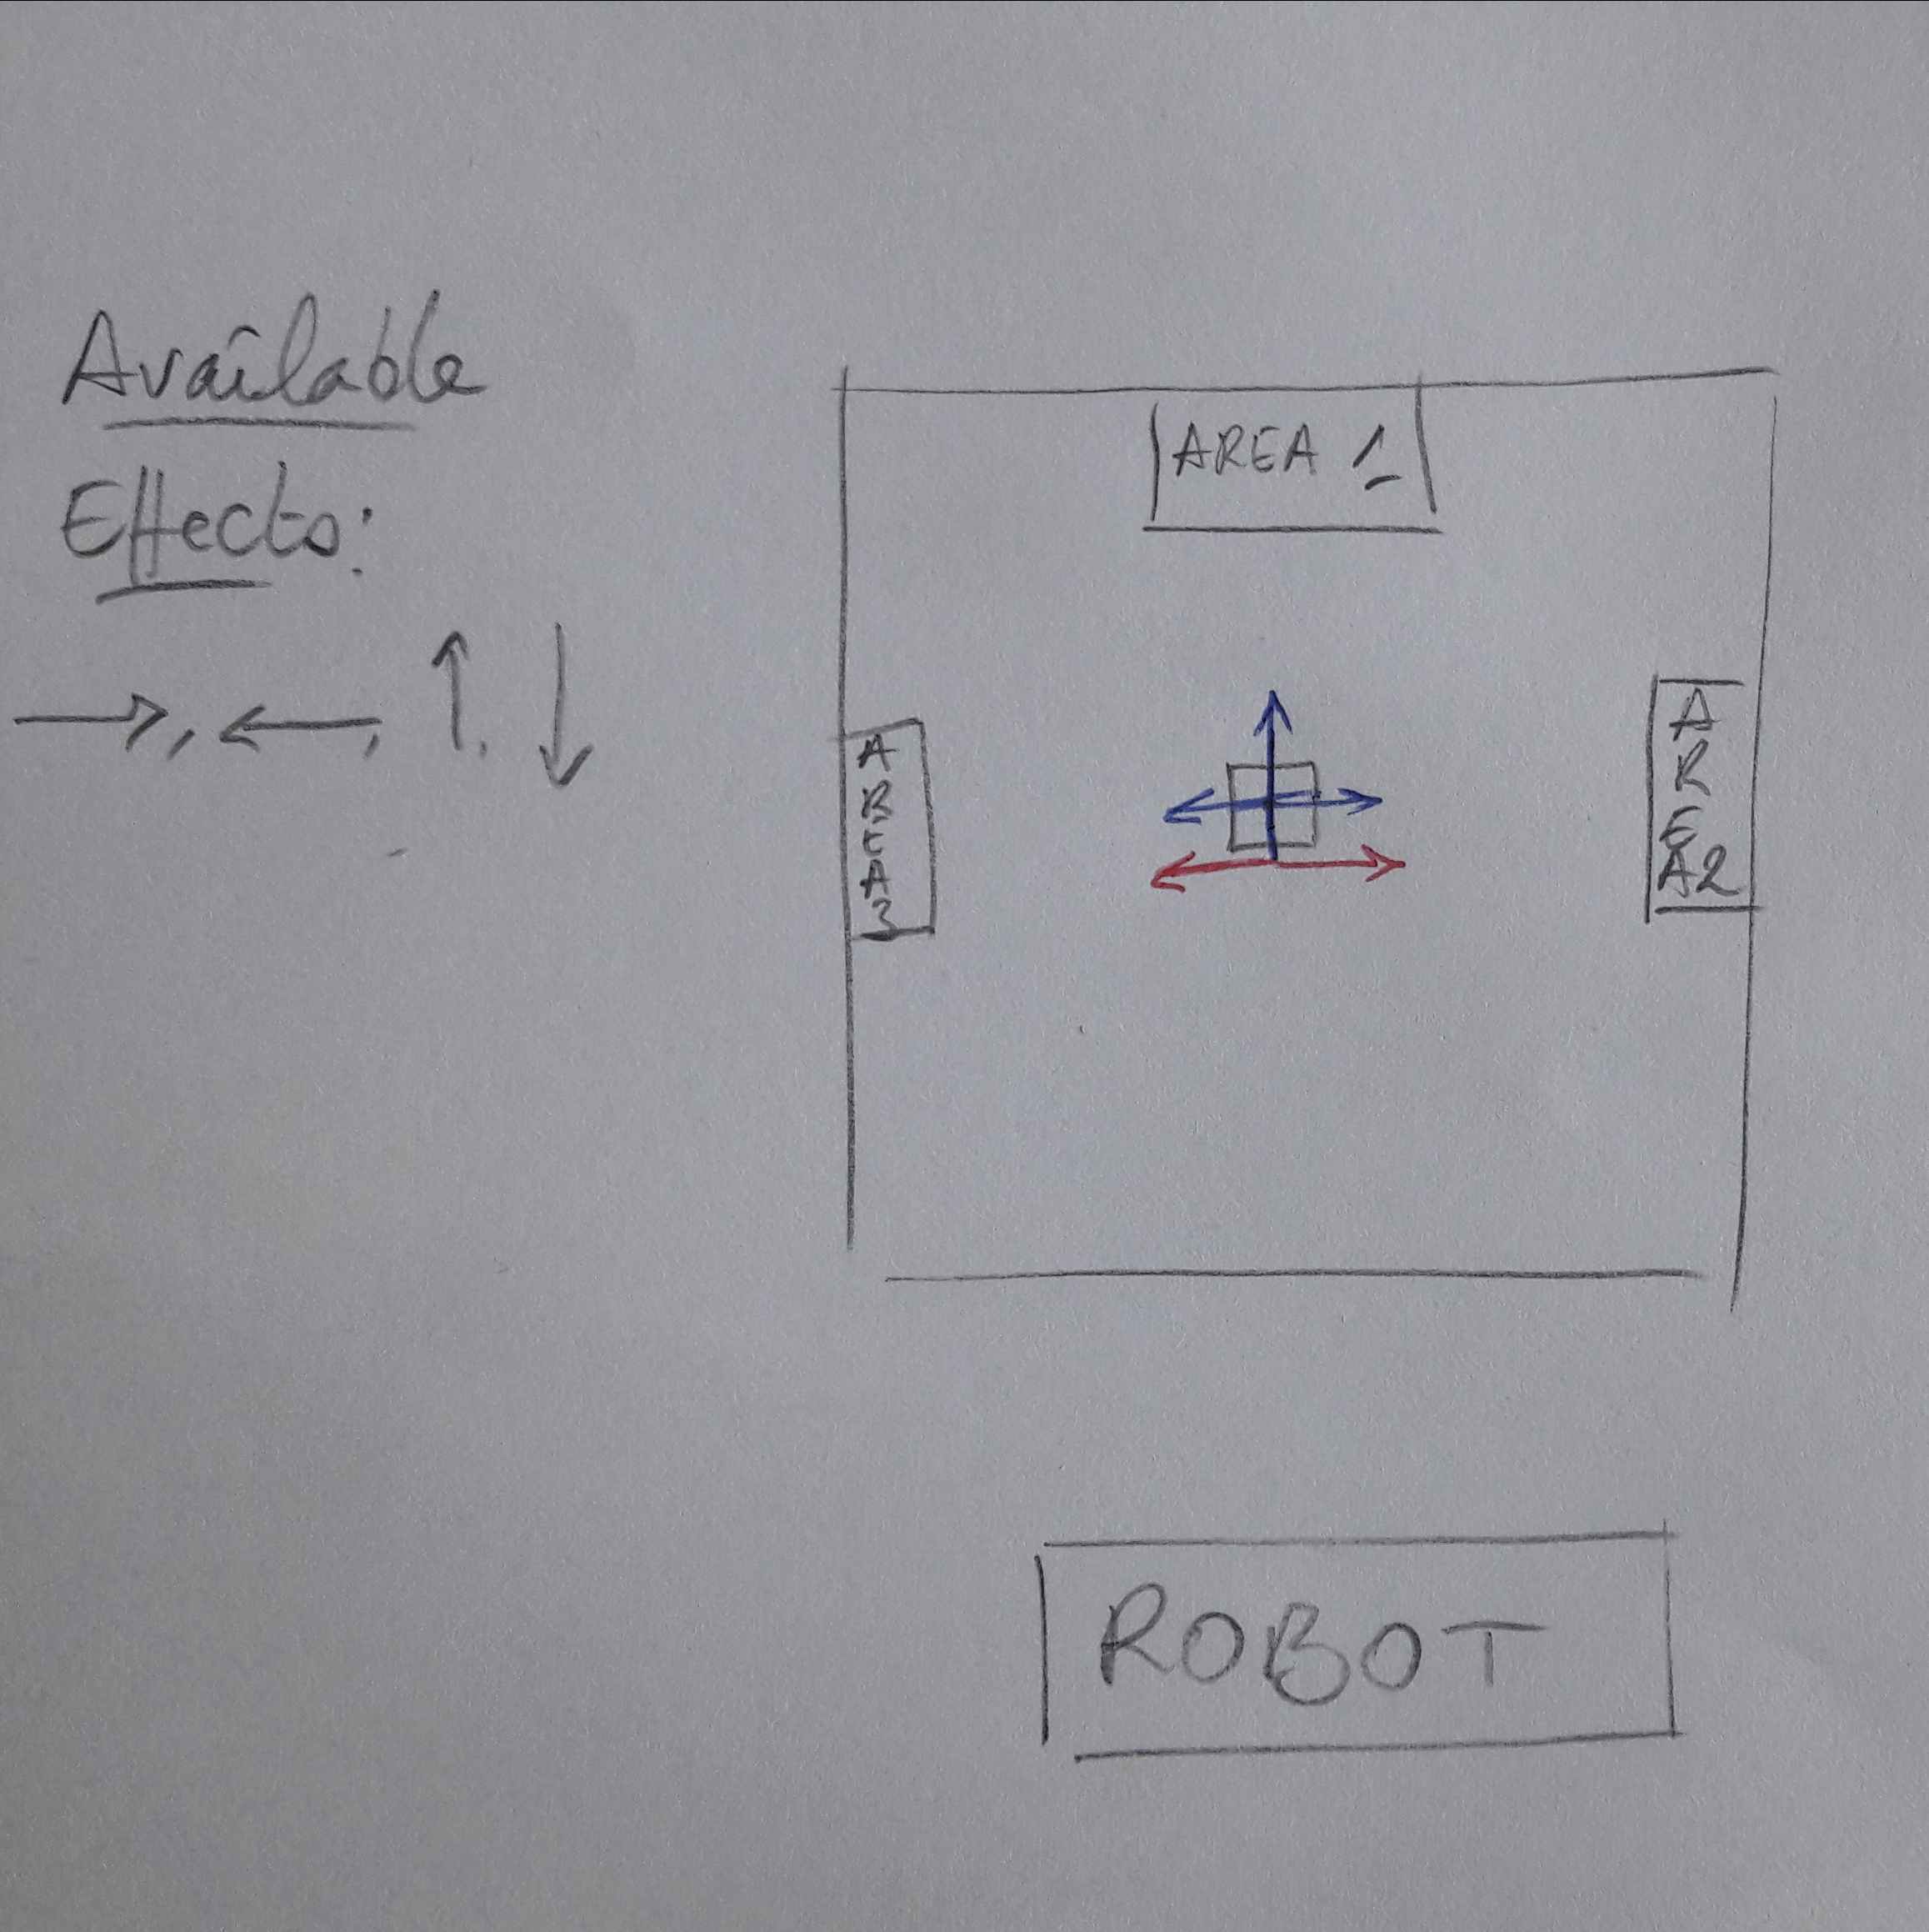
\includegraphics[width=0.4\textwidth]{figures/contact_position.jpg}
%     \caption{Les coordonnées du point de contact de l'effecteur sur l'objet permettent de positionner correctement l'effecteur lors de la phase de poussée. Cette indication est d'autant plus importante avec des objets ayant des propriétés particulières (cylindre, cône).}
%   \label{fig:contact_position}
%   \end{center}
% \end{figure}

% \begin{figure}[ht]
%   \begin{center}
%   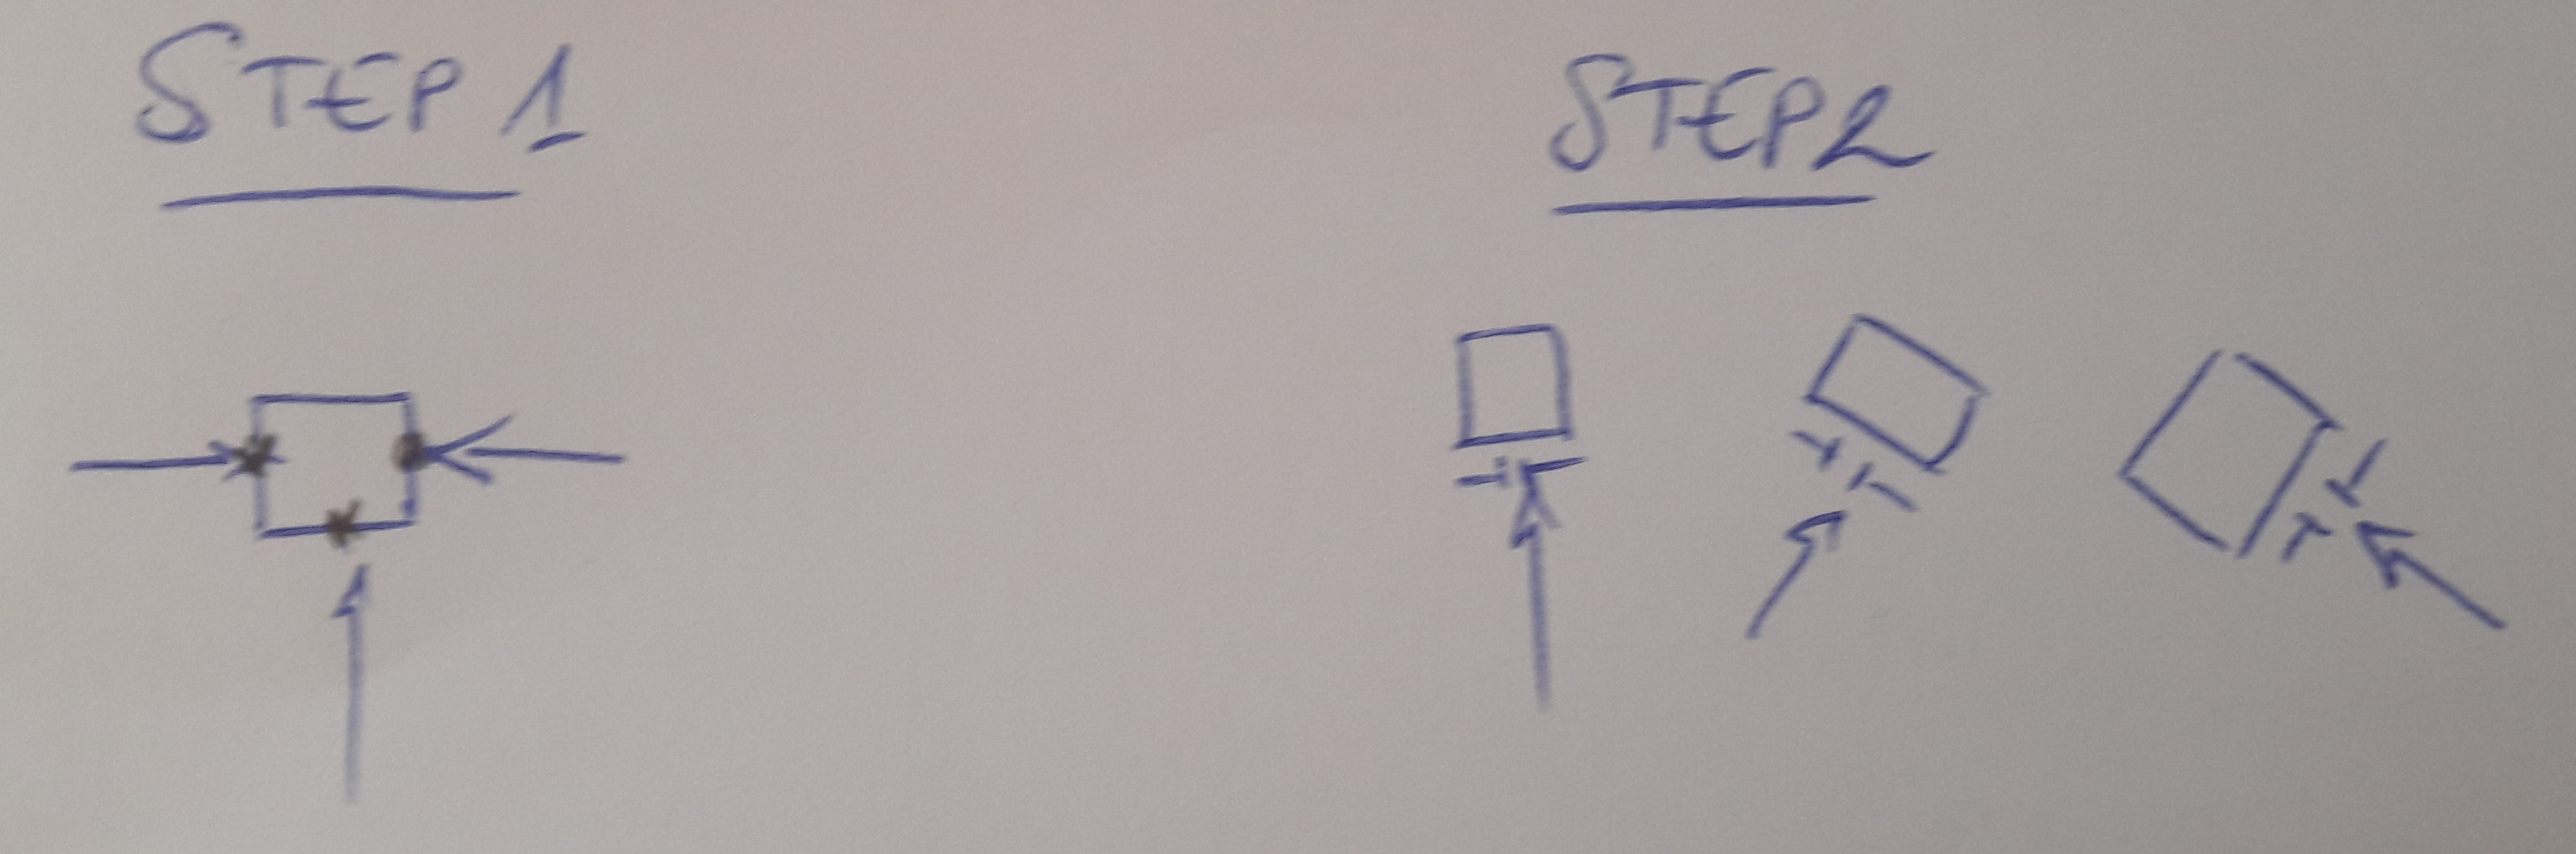
\includegraphics[width=0.6\textwidth]{figures/effector_problems.jpg}
%     \caption{Les coordonnées du point de contact de l'effecteur sur l'objet permettent de positionner correctement l'effecteur lors de la phase de poussée. Cette indication est d'autant plus importante avec des objets ayant des propriétés particulières (cylindre, cône).}
%   \label{fig:effector_problems}
%   \end{center}
% \end{figure}

Le premier problème provient du fait que les différents mouvements réalisés par le robot ne sont pas tous identiques.
Certains effectuent une poussée au milieu de la face considérée tandis que d'autres vont toucher cette même face à des positions très variées, parfois même aux extrémités de celle-ci.
Un mouvement au centre de la face a pour effet de pousser de manière rectiligne l'objet tandis qu'un mouvement en dehors de ce centre peut provoquer une rotation de l'objet sur l'axe $z$ en plus d'une trajectoire rectiligne.
Il convenait donc d'orienter l'effecteur pour qu'il se retrouve dans une configuration idéale, c'est-à-dire parallèle à la face considérée, avant tout mouvement.

Le second problème a trait avec la tâche elle-même.
En effet, dans un second temps de l'expérimentation, l'objet doit être poussé dans une zone inaccessible au bras du robot.
Cela signifie que l'objectif visé n'est pas simplement de pousser  un objet jusqu'à une zone particulière, mais d'effectuer un geste avec une vélocité élevée afin de pousser fortement l'objet jusqu'à cette zone.
L'utilisation de Quality Diversity doit pouvoir permettre d'effectuer un babillage relatif à la vélocité des lancers.





\subsubsection{Résultats}

Les premiers résultats provenant de cette expérimentation en simulation montrent que le robot est capable de pousser un objet vers une zone particulière accessible par le robot en se basant sur la discrétisation d'effets.
Afin de pousser l'objet dans la direction adéquate, le robot positionne son bras dans le sens opposé au déplacement.
Le robot effectue ensuite un déplacement correspondant à l'effet choisi et continue jusqu'à ce que l'objet se trouve dans la zone souhaitée.

Une vidéo de ces résultats est disponible en ligne : https://youtu.be/bKCBSDx8L1I





\section{Travaux futurs et perspectives}

\lettrine{P}{lusieurs} axes d'améliorations peuvent être proposés.
Durant ce stage, nous avons testé l'algorithme présenté ci-dessus avec un seul algorithme de clustering, \textit{Mean Shift}.
Le premier axe d'amélioration consisterait à tester davantage d'algorithmes de clustering, tels qu'\textit{Affinity Propagation}, \textit{Birch} ou \textit{DBSCAN}.

Un second axe d'amélioration pourrait être de tester l'algorithme avec des tâches plus complexes.
Par exemple. l'expérience pourrait consister à pousser l'objet dans une zone hors de portée du bras du robot.
Cette expérimentation nécessiterait l'utilisation d'algorithme de \textit{Quality Diversity} \cite{Pugh2016} pour générer un ensemble complet de déplacements.
Au sein de l'équipe AMAC, ce type particulier d'algorithmes est utilisé pour générer des trajectoires qui permettent au Baxter de lancer une balle dans un seau \cite{Kim2017}. 

Un troisième axe concerne l'expérience utilisant la clusterisation d'effets.
Il pourrait être pertinent de la réaliser en utilisant d'autres objets ayant différentes propriétés : un cylindre et un cône.
En effet, un cylindre a pour particularité de rouler sur une grande distance rectiligne lorsqu'il est poussé depuis sa face courbe alors que ce mouvement est plus réduit lorsqu'il est poussé depuis l'une de ses bases.
À l'inverse, un cône décrit une courbe s'il est poussé depuis sa face courbe et nécessite d'être poussé depuis sa base pour parcourir une grande distance rectiligne. 
Un babillage avec ces deux objets pourrait permettre au robot d'apprendre à repositionner les objets afin d'exposer leur face appropriée aux différentes actions (face courbe pour le cylindre et base pour le cône).

L'algorithme décrit dans ce mémoire a été utilisé pour une expérience réalisée en collaboration avec UDC et ISIR en vue de la réunion d'évaluation du projet DREAM qui se tient mi-septembre à Paris. 
Le but de cette expérience consiste à faire en sorte qu'un robot mobile puisse atteindre successivement différentes zones matérialisées par des puces RFID.
Pour cela, des techniques de Reinforcement Learning ont été utilisées conjointement avec l'algorithme de clusterisation d'effets.
Par ailleurs, cet algorithme peut être utilisé en amont du projet DREAM dans des travaux nécessitant une discrétisation de l'environnement.





\section{Conclusion}



% Qu'avez vous tiré de votre stage ?
\lettrine{A}{près} l'introduction donnée durant mon semestre de cours à Lyon, ce stage de Master 2 m'a permis de davantage découvrir le domaine de la robotique développementale 
Ce domaine de recherche, à la croisée de la robotique, de l'informatique et des neurosciences est un domaine riche, en plus d'être fascinant et très intéressant.
Les chercheurs s'emploient à créer des robots qui pourraient boostrap à partir d'une connaissance presque nulle de l'environnement.
Le lien étroit entre neurosciences (et spécialement neurosciences cognitives) permet d'implémenter des modèles présent chez l'être humain.
Le sujet abordé dans ce stage pointe la difficulté que représente la conception d'un robot autonome et capable d'apprendre en permanence dans son environnement.
Découvrir davantage le domaine de la robotique développementale.
Ce stage de six mois m'a également permis de côtoyer concrètement le monde de la recherche.
C'est un domaine exigeant qui nécessite d'être curieux et ouvert.

% Qu'avez-vous apporté à l'entreprise ?
% Développé un algorithme de clusterisation d'effets utilisables par l'équipe et les partenaires du projet DREAM.
Durant ce stage de six mois, nous avons proposé une approche qui permet à un robot d'apprendre depuis ses propres expériences et d'exploiter les données issues du babillage afin d'identifier des ensembles d'effets qui définissent des actions pertinentes pour un contexte dépendant de la tâche à accomplir.
Cet algorithme constitue un élément du projet DREAM qui pourra être utilisé par les différents partenaires et l'équipe AMAC.

% Qu'avez-vous acquis ? (méthodes de travail, rigueur, organisation, compétences, connaissances...)
Durant ce stage, j'ai développé un vaste ensemble de compétences nécessaires à la programmation de robots, notamment grâce à l'utilisation de frameworks et d'outils open source.
Le thème de mon stage m'a également amené à acquérir des connaissances solides dans le domaine de l'apprentissage d'affordances, tant d'un point de vue des neurosciences que du point vue de la robotique.

% Avez-vous atteint les objectifs que vous vous étiez fixés ? 
% Estimez-vous que vous avez réussi vos missions dans les temps impartis ?
L'avancement de mon stage, se terminant fin septembre, est conforme avec les jalons posés en début de stage.
La partie théorique contenant l'algorithme de clusterisation d'effets est achevée tout comme la partie concernant l'expérimentation en simulation.
Le mois restant sera consacrée à mise en place de l'expérimentation avec le robot réel et la constitution d'un benchmark en vue de la publication d'un nouvel article.

% Dans l'absolu, souhaiteriez-vous travailler dans ce genre d'entreprise ?
% Ce stage vous a-t-il apporté une orientation professionnelle plus précise ?
% A-t-il confirmé ou infirmé vos choix ? A-t-il fait naître d'autres désirs ?
Enfin, ce stage a confirmé mon choix de poursuivre en thèse après mon Master 2.
La recherche m'attire parce qu'elle est riche de savoirs et en constante progression.
Le domaine de la robotique développementale m'intéresse beaucoup parce qu'il est prometteur.
Cependant, je discerne que je souhaiterai davantage travailler dans un domaine moins fondamental et empirique, et avec davantage de modèles théoriques mathématiques.




% \section*{Annexe}

% Liste des différentes waves

% \begin{tabular}{|l|c|r|}
%   \hline
%   No & Requirements 2 & Partners \\
%   \hline
%   W1 & Babbling & UPMC \\
%   W2 & Saliency Learning & UPMC \\
%   W2 & Saliency Learning & UPMC \\
%   W3 & Object Babbling & UPMC \\
%   W4 & Object Interaction Babbling & UPMC \\
%   W5 & Object Interaction discretization & UPMC \\
%   W6a & End to End policy pre-training & QMUL \\
%   W6b & End to End policy fine tuning & QMUL \\
%   W7 & Feature learning & Armines \\
%   W8 & Feature Based Reinforcement Learning & Armines \\
%   W9 & Policy-based exploration & Armines \\
%   W10 & Contextual Policy learning & UPMC \\
%   W11 & Model learning & UDC \\
%   W12 & Value function learning & UDC \\
%   W13 & Policy modularization & QMUL \\
%   \hline
% \end{tabular}

% Liste des différentes working packages

% \begin{tabular}{|l|c|r|}
%   \hline
%   No & Requirements 2 & Partners \\
%   \hline
%   W1 & Babbling & UPMC \\
%   W2 & Saliency Learning & UPMC \\
%   W2 & Saliency Learning & UPMC \\
%   W3 & Object Babbling & UPMC \\
%   W4 & Object Interaction Babbling & UPMC \\
%   W5 & Object Interaction discretization & UPMC \\
%   W6a & End to End policy pre-training & QMUL \\
%   W6b & End to End policy fine tuning & QMUL \\
%   W7 & Feature learning & Armines \\
%   W8 & Feature Based Reinforcement Learning & Armines \\
%   W9 & Policy-based exploration & Armines \\
%   W10 & Contextual Policy learning & UPMC \\
%   W11 & Model learning & UDC \\
%   W12 & Value function learning & UDC \\
%   W13 & Policy modularization & QMUL \\
%   \hline
% \end{tabular}

% % \addcontentsline{toc}{chapter}{Annex}
%
% % \begin{tabular}{|l|c|r|}
% %   \hline
% %   colonne 1 & colonne 2 & colonne 3 \\
% %   \hline
% %   1.1 & 1.2 & 1.3 \\
% %   2.1 & 2.2 & 2.3 \\
% %   \hline
% % \end{tabular}
%
% \begin{tabular}{ |l|l|l| }
% % \hline
% % \multicolumn{3}{ |c| }{Team sheet} \\
% \hline
% Type & Name & Since \\ \hline
% \multirow{4}{*}{Partitionnement} & LB & Lucas Radebe \\
%  & DC & Michael Duburry \\
%  & DC & Dominic Matteo \\
%  & RB & Didier Domi \\ \hline
% \multirow{3}{*}{Basé sur la densité} & MC & David Batty \\
%  & MC & Eirik Bakke \\
%  & MC & Jody Morris \\ \hline
% \multirow{2}{*}{Grid based} & ST & Alan Smith \\
%  & ST & Mark Viduka \\
% \hline
% \end{tabular}

\bibliographystyle{unsrt}
\bibliography{./LEROY_M2_ISIR_2017_internship_thesis.bib}

\end{document}
